\documentclass{article}
\usepackage{tmlr}
% \usepackage[accepted]{tmlr}   % camera-ready
\usepackage{amsmath,amssymb,amsthm}
\usepackage{booktabs}
\usepackage{graphicx}
\usepackage{xcolor}
\usepackage{hyperref}
\usepackage{url}
\usepackage{multirow}

\newtheorem{proposition}{Proposition}
\newtheorem{remark}{Remark}
\newcommand{\eps}{\varepsilon}
\newcommand{\ACT}{\mathrm{ACT}}
\newcommand{\Jfifty}{J_{50}}

\title{Certifying Retrieval-Policy Deployment with Non-Neutral AI Judges:\\ Decision Weights, Control Variates, and What Judge Accuracy Does Not Tell You}

\author{\name Anonymous authors \\ \addr Paper under double-blind review}

\begin{document}
\maketitle

\begin{abstract}
Before a retrieval policy is deployed in a new domain, an auditor must certify from a limited human audit that it is within a tolerance $\eps$ of the best alternative. LLM relevance judges can label every candidate document, but a judge may be biased toward one of the policies it judges. We ask which judge helps the human audit, by how much, and whether the certificate can still be trusted, for menus of cutoff policies over a shared candidate pool (set-F1 or precision utilities) on eight retrieval collections, five AI judges, and three pre-registered evaluations. (i)~What a judge is worth is not its label accuracy but the correlation $\rho$ between true and judge-predicted \emph{paired policy differences}: over 54 (collection, pair, judge) settings the realised gain of prediction-powered inference correlates $0.75$ with $\rho$ and $0.03$ with accuracy. A mechanism map shows that a certificate gains only from judges with $\rho\ge0.57$, only at tolerances the human audit cannot settle alone, and more the larger the unlabeled pool. A judge built from the model that defines a policy over-credits it by $0.14$~F1; this mean bias is removed exactly by the correction and is distinct from the loss of $\rho$ that governs efficiency. (ii)~In a sample-split certificate the judge enters only as a mean-zero control variate, so no judge biases the estimator of any fixed policy contrast, and a data-dependent candidate is covered by simultaneous bounds over the fixed family of contrasts. Coverage rests on the bound applied to the corrected differences: the one-sided $t$ bound we use is asymptotically calibrated, with observed wrong-certificate rates $\le0.008$ in development and $0/500$ to $6/500$ in the pre-registered evaluations; a finite-sample-exact betting certificate is affordable on two collections and close to a census on two others because of its range term. (iii)~Defining the estimand yields closed-form per-document \emph{decision weights}. With every unique human label charged once, pilot included, importance sampling by these weights needs $40$--$56\%$ fewer labels than uniform document sampling in a fixed-budget design (a joint effect of skipping documents no comparison depends on and of weighting the rest); a $\lambda$-fitted judge control variate saves a further 3--20\% when its $\rho$ is high and nothing beyond noise otherwise; a faithful active-inference rule matches it within noise; and optimising the allocation across the comparisons of a menu saves only 0--14\% even for an oracle, because the pilot's candidate choice and the decision margin set the cost. We claim no new estimation theory: the contribution is the exact mapping of policy certification onto existing inference tools, the measured conditions under which judges pay, a cost accounting that charges every label once, and three pre-registered evaluations in which validity replicated every time while the efficiency criteria did not, each for a reason we name.
\end{abstract}

\section{Introduction}
Retrieval systems are increasingly deployed as configurable policies: a fixed ranker plus a rule that decides how many documents to return, which threshold to apply, or which reranker to trust. When such a system moves to a new domain, an auditor with a small human-judgment budget must decide whether a candidate policy can be deployed---formally, whether its utility is within $\eps$ of the best alternative on the target distribution---or whether to collect more judgments or abstain. Two developments make this problem timely. First, LLM relevance judges are cheap enough to label every candidate document, so the audit can be assisted by a judge. Second, the policies themselves are often built from the same model families as the judges, so a judge may not be neutral toward the policies it evaluates \citep{balog2025rankers}.

Prediction-powered inference (PPI) and active statistical inference provide the statistical machinery for combining AI predictions with human labels \citep{angelopoulos2023ppi,angelopoulos2023ppipp,zrnic2024active}. Applied naively, however, they leave three questions open that an auditor must answer before spending a budget: \emph{which} judge to use, \emph{whether} the resulting certificate can be trusted if the judge is wrong or biased, and \emph{where} to spend the human labels. This paper answers all three for the policy-certification problem, and reports what happened when the answers were tested on data that had been locked before analysis.

\paragraph{Contributions.}
\begin{enumerate}
\item \textbf{What a judge is worth is not its accuracy.} For paired policy differences with $n$ audited and $N$ unlabeled queries, the PPI++ effective-sample-size gain at the optimal coefficient is $1/(1-\rho^2/(1+n/N))$, i.e.\ $1/(1-\rho^2)$ when $N\gg n$, where $\rho$ is the correlation of true and predicted differences (Proposition~\ref{prop:A}, a restatement of PPI++ for this problem). Across 54 (collection, pair, judge) settings the realised gain, measured as the ratio of squared estimated standard errors, correlates $0.75$ with $\rho$ and $0.03$ with pair-level judge accuracy; the relation holds within 13 of the 14 (collection, judge) groups and for every judge swap at fixed policies (Section~\ref{sec:judge}). A mechanism map on real data (Figure~\ref{fig:F6}) shows that the certificate gains only from the judges with $\rho\ge0.57$, only at tolerances the human-only certificate cannot settle easily, and more the larger the unlabeled pool. A judge built from the model that defines a policy over-credits that policy by $0.14$ on paired F1; we separate this mean bias, which the correction removes exactly, from the loss of $\rho$ for that policy's comparisons ($0.57\to0.25$), which every judge shows and which is what costs efficiency (Section~\ref{sec:selfpref}).
\item \textbf{A certificate whose estimator no judge can bias.} Splitting the audit into a training half (policy parameters, judge adoption) and a validation half (the bound) makes the certificate valid conditionally on every choice made on the training half, and the judge enters only through a control variate whose mean is zero, so no judge---however biased---can bias the estimator; the coverage of the certificate depends only on the level of the bound applied to the corrected differences (Proposition~\ref{prop:B}). Two things are therefore kept apart throughout: the \emph{unbiasedness} of the judge-corrected estimator, which holds for every judge, and the \emph{coverage} of the confidence bound, which depends on the bound's own hypothesis. The implementation uses a one-sided $t$ bound and is therefore asymptotically, not finite-sample, calibrated; we show empirically that the earlier in-sample certificate exceeded its nominal risk, that the split certificate stays at $\le 0.008$ observed wrong certificates across 24 cells and at $0/500$ under an adversarial judge, and that an \emph{always-use-the-judge} policy can lose efficiency with a poor judge while a pilot-based adoption rule protects it. We then price exactness: a finite-population $t$ certificate for the fixed evaluation set stops 20--27\% earlier than the pre-registered one, while an exact without-replacement betting certificate is practical only where the margin or the population is large---at $\eps=0.01$ it fires by 75\% of the population in 73--90\% of runs on two collections and in 0--2\% on the other two, where it fires almost only at budgets close to a census (Section~\ref{sec:valid}).
\item \textbf{Where to spend human judgments.} For utilities with a label-independent normaliser, the paired difference is a linear functional with closed-form per-document decision weights (Proposition~\ref{prop:C}); the common documents carry weight $|1/k_a-1/k_b|$, so a band-only audit is exact only when cutoffs coincide. With every unique human label charged once (pilot included, one label serving all comparisons of the menu) and in a fixed-budget design, importance sampling by these weights roughly halves the labels needed to certify relative to uniform sampling on four collections ($-40$ to $-56\%$; a joint effect of not labelling documents that no comparison depends on and of weighting the rest, which Table~\ref{tab:J50} does not separate); a $\lambda$-fitted judge control variate adds 3--20\% of the total cost (16--35\% of the post-pilot labels) when the judge's $\rho$ is high and nothing beyond noise when it is not; a faithful active-inference rule matches this within noise; the calibrated-judge rule is the only arm an adversarial judge breaks (Section~\ref{sec:where}). An exact minimax allocation of labels across the comparisons of the menu, solved with oracle knowledge, saves only 0--14\%, and we separate the two reasons (Section~\ref{sec:negative}). For set-F1 we give a bias-corrected linearisation and measure its remainder (Appendix~\ref{app:f1}).
\item \textbf{Three pre-registered external evaluations.} On TREC Deep Learning 2021--2023 (211 queries) the query-level methods, on TREC CAsT 2019 (159 conversational turns) the document-level methods, and on ANTIQUE (200 non-factoid questions) the $\lambda$-corrected control variate were evaluated under locks committed before the data were touched. Validity replicated every time (wrong certificates $0/500$, $0/500$ and $\le6/500$; boundary type-I error $\le0.013$). The pre-registered efficiency criteria were not met in any of the three, each time for a reason we can name---too small a $\rho$ and unlabeled pool, too small a budget grid, a saturated one---and we report all three as is (Section~\ref{sec:prereg}). The CAsT evaluation exposed a defect of the coefficient-1 control variate under an adversarial judge; the ANTIQUE evaluation confirmed the $\lambda$-corrected fix.
\end{enumerate}

\paragraph{What we do not claim.} We do not propose a new estimator or a new sampling optimality result; our estimator is a special case of active inference for a linear functional (Section~\ref{sec:relation}). We do not claim that AI judges reduce audit cost unconditionally; the pre-registered evaluation shows they need not. We do not claim a general theory of judge neutrality; the self-preference signature we measure is specific to the identical-model judge.

\section{Setup}\label{sec:setup}
Let $P$ be the target query distribution, $\mathcal{M}$ a finite menu of policies acting on a shared ranked candidate pool for each query $q$, and $u_m(q)\in[0,1]$ the utility of policy $m$ on $q$ given human relevance labels $y_d\in\{0,1\}$ for the pooled documents $d$. Two utilities are used: set-F1, $u_m(q)=2\,\mathrm{tp}_m/(k_m+n_G)$ with $k_m=|R_m(q)|$ and $n_G(q)=\sum_d y_d$, and precision at the policy's cutoff, $u_m(q)=\mathrm{tp}_m/k_m$. Population utilities are $\mu_m=\mathbb{E}_P[u_m(q)]$.

\paragraph{Decision and error.} A certificate $\ACT$ selects a candidate $\hat m$ and asserts $\max_{j}\mu_j-\mu_{\hat m}\le\eps$. A \emph{wrong certificate} is an $\ACT$ whose true regret exceeds $\eps$. All methods use the same risk budget: for looks $t=1..L$ and ordered pairs $(j,\hat m)$, each one-sided upper confidence bound $U_{t,j}$ on $\mu_j-\mu_{\hat m}$ is at level $1-\alpha'$ with $\alpha'=\alpha/(L\,|\mathcal M|(|\mathcal M|-1))$, and $\ACT_t\iff\max_{j\ne\hat m}U_{t,j}\le\eps$ ($L=1$ in the fixed-budget designs of Section~\ref{sec:where}). Throughout $\alpha=0.10$; $\eps\in\{0.005,0.01,0.02,0.05\}$.

\paragraph{Audit units and the judge.} A \emph{query-level} audit labels a query's whole pool (needed for set-F1 because of $n_G$); a \emph{document-level} audit labels a sampled subset of documents. An AI judge is a fixed map $f$ from a (query, document) pair to a relevance probability; we threshold it at $0.5$ for judge utilities $\hat u_m(q)$ and use the probability where a rule requires it. Nothing below assumes the judge is calibrated, unbiased, or independent of the policies.

\paragraph{Efficiency metric.} Two designs are used and their costs are defined separately. In the \emph{sequential} query-level design (Sections~\ref{sec:valid} and \ref{sec:prereg}) one audit path is followed through the looks $t=1..L$ at the level $\alpha'$ above, and we report the cumulative $\ACT$ rate at each look. In the \emph{fixed-budget} document-level design (Section~\ref{sec:where}) each budget is a separate audit with its own pilot and sample, evaluated once ($L=1$), and we report the probability of certifying at that budget; $\Jfifty$ is the budget---in unique human-judged (query, document) pairs, every label consumed included (pilot/training queries, judge selection, residual models, and the bound itself)---at which this probability first reaches 50\%, interpolated linearly between the budgets actually run. $\Jfifty$ is therefore the cost of a pre-committed budget that certifies half the time; it is not the expected stopping cost of a procedure that inspects several budgets, which would need labels accumulated along one path and an error control over looks that the document-level runs do not implement. A cell whose largest budget stays below 50\% is reported as \emph{not reached} and never enters a ratio. Wrong-certificate rates are reported next to every $\Jfifty$ with Clopper--Pearson 95\% intervals. Query-level (set-F1) and document-level (precision) blocks use different utilities and are never compared to each other.

\section{What determines the value of a judge}\label{sec:judge}
\begin{proposition}[PPI gain for paired differences]\label{prop:A}
Fix policies $j,m$ and let $D=u_j-u_m$, $\hat D=\hat u_j-\hat u_m$ with variances $\sigma^2,\hat\sigma^2$ and correlation $\rho$. With $n$ audited and $N$ unlabeled queries drawn independently, the PPI++ estimator $\hat\mu(\lambda)=\lambda\,\overline{\hat D}_N+\overline{(D-\lambda\hat D)}_n$ has variance $[\sigma^2-2\lambda\rho\sigma\hat\sigma+\lambda^2\hat\sigma^2]/n+\lambda^2\hat\sigma^2/N$, minimised over unconstrained $\lambda$ at $\lambda^\star=\rho\sigma/\big(\hat\sigma\,(1+n/N)\big)$ to $\frac{\sigma^2}{n}\big(1-\frac{\rho^2}{1+n/N}\big)$. The effective-sample-size gain over the human-only estimator is therefore $G=1/\big(1-\rho^2/(1+n/N)\big)$, which increases to $1/(1-\rho^2)$ as $N/n\to\infty$: at the optimal coefficient the judge enters only through $\rho$ and the ratio $n/N$.
\end{proposition}
The proof is a direct variance computation (Appendix~\ref{app:proofs}); the statement is PPI++ \citep{angelopoulos2023ppipp} applied to a paired difference, and we use it as the reference curve of Figure~\ref{fig:F4}, not as a new result. Three qualifications matter for reading the experiments. First, $G$ is the gain at the oracle $\lambda^\star$; the implementation estimates $\lambda$ by cross-fitting on halves of the audited queries, and the estimation noise costs part of the gain at small $n$ (Section~\ref{sec:valid}). Second, the implementation clips $\lambda$ to $[0,1]$: a judge whose $\hat D$ is negatively correlated with $D$ would help an unconstrained estimator but is simply switched off ($\lambda=0$), and when $\rho\sigma/\hat\sigma$ exceeds $1+n/N$ the clipped $\lambda=1$ delivers less than $G$. Third, the proposition is about the variance of an estimator; whether a certificate fires is a threshold event on a bound, and Figure~\ref{fig:F6} measures that separately.

\paragraph{Bias toward a policy and $\rho$ are different quantities.} It is tempting to read Proposition~\ref{prop:A} as ``a judge biased toward one policy has a low $\rho$''. Writing $\hat u_m=u_m+b_m+e_m$ with a policy-specific bias $b_m$ and a query-level error $e_m$, $\hat D=D+(b_j-b_m)+(e_j-e_m)$. A constant $b_j-b_m$, however large, shifts every $\hat D$ by the same amount and leaves $\rho$ unchanged ($\hat D=D+0.1$ has $\rho=1$), and it is removed exactly by the control variate of Section~\ref{sec:valid}. What lowers $\rho$ is the query-varying part $(b_j(q)-b_m(q))+(e_j-e_m)$ relative to $\mathrm{Var}(D)$, together with its covariance with $D$. Bias toward a policy therefore has two separate consequences that the paper keeps apart: a \emph{mean bias}, which corrupts any judge-only comparison of the policies (Section~\ref{sec:selfpref} measures $0.14$~F1 for the identical-model judge) but not the corrected estimator, and a \emph{loss of predictive correlation}, which reduces the gain the judge can deliver once corrected. The second need not accompany the first: in Section~\ref{sec:selfpref} the drop in $\rho$ for the reranker-defined policy appears for every judge, biased or not, and the judge with the largest mean bias is not the one with the lowest $\rho$ on the other pairs.

\paragraph{Empirical test.} We measured $\rho$ and the realised gain---the ratio of the squared estimated standard errors of the human-only and PPI++ estimators, averaged over random audits (cross-fitted $\lambda$, $T=10$ audited queries, 300 random audits)--- on 54 (collection, pair, judge) settings: four BEIR development pools under a legacy and a modern retrieval stack, five fully judged pools (TREC DL 2019, 2020; TREC-COVID; Touch\'e~2020; DBpedia-Entity), and two judges (Qwen3-Reranker-0.6B and Qwen3-8B with the UMBRELA prompt). Figure~\ref{fig:F4} shows the result: $\mathrm{corr}(\text{gain},\rho)=0.75$ and $\mathrm{corr}(\text{gain},\text{pair accuracy})=0.03$ (all figures in this paragraph are regenerated from the released result files by \texttt{93\_plot\_F4.py}). The relation is not an artefact of pooling heterogeneous groups: demeaned within the 14 (collection, judge) groups it is $0.66$ and positive in 13 of the 14 (the exception is cqadupstack-android with the reranker, where every $\rho$ lies between $-0.17$ and $0.07$ and every gain below one, so there is no relation to detect); and for the 13 (collection, pair) settings in which switching from the reranker to the LLM judge raised $\rho$, the gain rose in all 13. The estimated-standard-error ratio is a proxy for the quantity of interest, the ratio of the estimators' mean squared errors about the population gap; on the 33 settings whose pools are in the released bundle (the four BEIR pools under both stacks and the three judged pools with the reranker judge) we re-measured both from 500 random audits per setting. The Monte-Carlo MSE ratio correlates $0.78$ with $\rho$ (the estimated-SE ratio $0.83$ on the same 33), the two agree to a median absolute difference of $0.03$, and where they differ the estimated-SE ratio understates the gain (TREC-COVID, $\rho\approx0.75$: MSE ratio $1.5$--$1.7$ against $1.1$--$1.2$). The two-sided $90\%$ intervals of both estimators cover the population gap at $0.90$ on average (minimum $0.81$ over settings, $T=10$). The 21 remaining settings (TREC DL 2019/2020 and the two LLM-judged BEIR pools) could not be re-measured because their pools and judge outputs are not in the bundle; for them only the estimated-SE ratio is reported.

\begin{figure}[t]\centering

\includegraphics[width=0.72\linewidth]{figures/F4_gain_vs_rho.png}
\caption{Realised PPI gain (ratio of squared estimated standard errors) at $T=10$ against $\rho$, 54 settings, cross-fitted $\lambda$. The dashed curve is $1/(1-\rho^2)$. Colour/marker distinguish pools and judges. Gains track $\rho$ (0.75) and not accuracy ($0.03$).}\label{fig:F4}
\end{figure}

\paragraph{When does the gain materialise?} Proposition~\ref{prop:A} concerns the variance of an estimator at the optimal $\lambda$; whether a certificate fires is a threshold event on a bound computed from the $T/2$ validation queries with an estimated $\lambda$. On DBpedia-Entity (399 queries) and TREC DL 2021--23 (211 queries) we manipulated three quantities: the judge's $\rho$ (by replacing a fraction $0$--$0.9$ of its labels with base-rate coin flips, giving $\rho=0.64,0.57,0.39,0.26$ on DBpedia-Entity), the unlabeled size $N_{\mathrm{unlab}}\in\{50,100,200,300\}$, and $\eps$, and measured the $\ACT$ ratio of the PPI certificate to the human-only certificate at $T=90$ (Figure~\ref{fig:F6}; 300 repeats per cell). Three regularities hold in the stored results. (a)~With $\rho\le0.39$ the ratio lies between $0.76$ and $1.06$ in every cell, whatever $N_{\mathrm{unlab}}$ and $\eps$. (b)~With $\rho\ge0.57$ and $\eps\le0.02$ the ratio exceeds $1.2$ in 11 of the 12 cells with $N_{\mathrm{unlab}}\ge200$ ($1.21$--$1.53$; the exception, $\rho=0.57$, $N_{\mathrm{unlab}}=300$, $\eps=0.02$, is $1.11$), and for $\rho=0.64$ already at $N_{\mathrm{unlab}}=100$ and $\eps=0.01$ ($1.38$); with $N_{\mathrm{unlab}}=50$ it never exceeds $1.17$, and at $\eps=0.05$, where humans alone certify roughly 90\% of runs, it is $0.95$--$1.01$ for every judge. (c)~Every cell has wrong-certificate rate $\le0.01$. We read the map as a description of where the gain appeared under these conditions, not as a universal threshold: the judge's $\rho$ is the first-order quantity, the unlabeled pool the second, and a tolerance that humans alone cannot settle is a precondition. On TREC DL 2021--23 the judge reaches $\rho\le0.46$ and $N_{\mathrm{unlab}}\le100$, and no cell has a ratio above $1.05$---which is exactly what the pre-registered evaluation found (Section~\ref{sec:prereg}). The map is not a collection-specific accident: running the same certificate code on Gaussian paired differences whose gaps, standard deviations and $\rho$ are read from the population (Appendix~\ref{app:calculator}) reproduces the 64 DBpedia-Entity cells with a correlation of $0.85$ between simulated and measured ratios (mean absolute error $0.06$; agreement on the $1.2$ threshold in 92\% of cells) and the 32 TREC DL cells with a mean absolute error of $0.03$, and it does so only with the cross-fitted $\lambda$: with the population-optimal $\lambda$ the losses of the poor judge on TREC DL disappear from the simulation (correlation $0.12$), so those losses are the price of estimating $\lambda$ on 22-query folds, not a property of the judge.

\begin{figure}[t]\centering
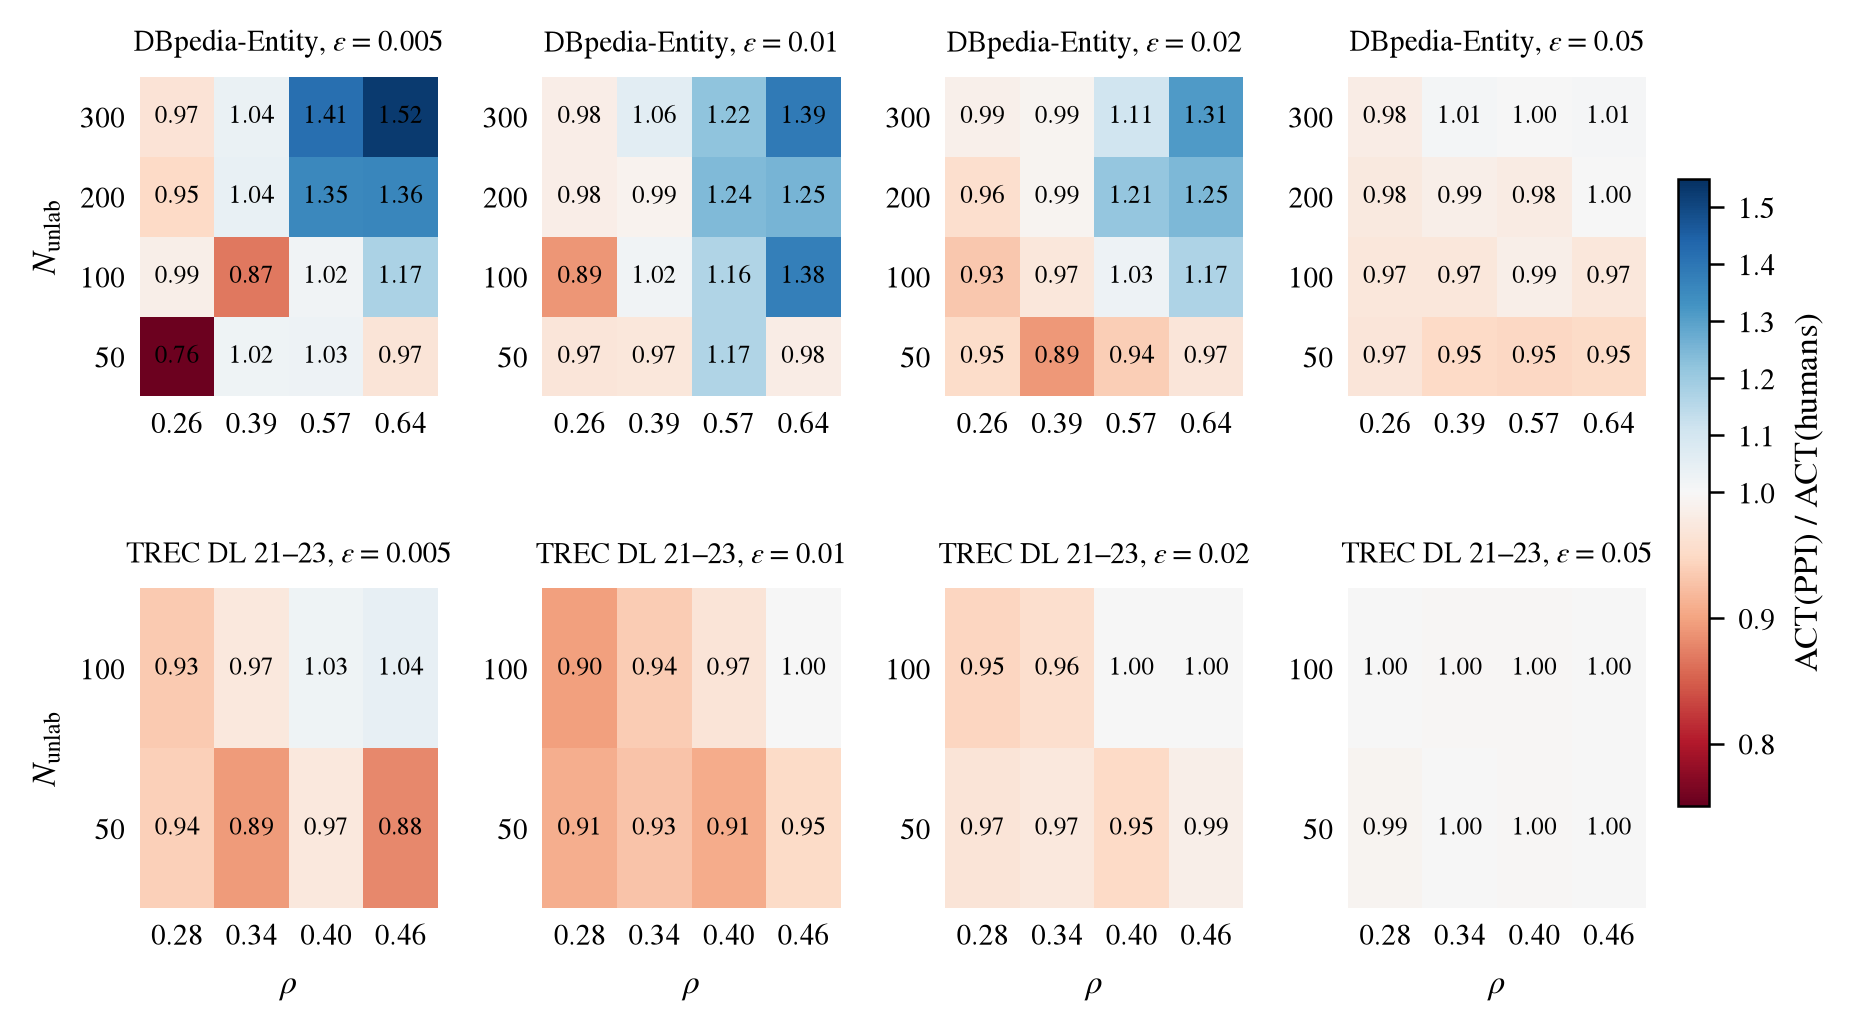
\includegraphics[width=\linewidth]{figures/F6_rho_map.png}
\caption{Mechanism map: $\ACT(\text{PPI})/\ACT(\text{humans})$ at $T=90$ over $\rho$ (judge-label noise), unlabeled pool size and $\eps$; wrong-certificate rate $\le0.01$ in every cell. Gains appear only for $\rho\ge0.57$ and $\eps\le0.02$, grow with $N_{\mathrm{unlab}}$, and are absent at $N_{\mathrm{unlab}}=50$ and at $\eps=0.05$.}\label{fig:F6}
\end{figure}

\subsection{Judges built from the model that defines a policy}\label{sec:selfpref}
We added to the menu a fourth policy, \texttt{rr\_thresh}, that returns every pooled document whose Qwen3-Reranker score exceeds a threshold tuned on the audit, so that one policy is defined by a model in the judges' family. With policies fixed at their population parameters, we compared five judges on the six policy pairs of five fully judged pools (Table~\ref{tab:selfpref}). Two signatures are specific to the \emph{identical-model} judge: it over-credits its own policy by $-0.14$ on the paired F1 difference (all other judges $-0.04$ to $+0.03$), and its error rate inside the documents on which the two policies disagree rises from $0.36$ to $0.41$. The drop in $\rho$ for pairs involving \texttt{rr\_thresh} appears for every judge, including the different-family MPNet rule, so it is largely a property of that policy's paired differences rather than of self-preference. Validity is unaffected: with the four-policy menu the split certificate produced $0/500$ wrong certificates for both the identical-model and the same-family judge, and the identical-model judge yielded no efficiency gain (ACT $246$ vs $245$ human-only) while the 8B judge did ($328$).

\begin{table}[t]\centering\footnotesize
\caption{Self-preference test at fixed policies: mean over 15 policy pairs per judge, split by whether the pair involves the reranker-defined policy (``without / with''). ``Bias'' is the mean of predicted minus true paired difference.}\label{tab:selfpref}
\begin{tabular}{lcccc}\toprule
Judge & $\rho$ & in-band / out-of-band error & bias & PPI gain\\\midrule
Qwen3-Reranker (identical model) & 0.57 / 0.25 & 0.36 / 0.32 $\to$ 0.41 / 0.31 & $-0.03$ / $\mathbf{-0.14}$ & 1.07 / 0.95\\
Qwen3-8B (same family) & 0.69 / 0.48 & 0.28 / 0.24 $\to$ 0.29 / 0.23 & $0.00$ / $-0.04$ & 1.19 / 1.04\\
Mistral-7B (other family) & 0.38 / 0.30 & 0.34 / 0.34 $\to$ 0.37 / 0.33 & $+0.02$ / $-0.04$ & 1.10 / 1.06\\
MPNet rank rule (other family) & 0.39 / 0.21 & 0.39 / 0.35 $\to$ 0.40 / 0.35 & $-0.05$ / $+0.03$ & 1.03 / 0.94\\\bottomrule
\end{tabular}
\end{table}

\section{A certificate whose bias does not depend on the judge}\label{sec:valid}
\paragraph{Why the earlier certificate was not.} The certificate used in our earlier development (leave-one-out cross-fitted utilities, paired bootstrap, Bonferroni over looks $\times(|\mathcal M|-1)$ comparisons) chose the candidate on the same data used for the bound. With exact $t$ bounds on synthetic data this alone raises the per-look miss rate from the $0.020$ budget to $0.049$; correcting over all $|\mathcal M|(|\mathcal M|-1)$ ordered pairs restores $0.014$. On real data at 500 repeats the earlier certificate's wrong-certificate rate was $0.146$ $[0.116,0.180]$ on one development pool and $0.180$ $[0.147,0.217]$ on another, both above $\alpha=0.10$ with the whole interval.

\paragraph{Split certificate.} At look $t$ the audited queries are split into a training half $A_t$ and a validation half $B_t$. Policy parameters and the decision whether to adopt the judge are made on $A_t$; the candidate $\hat m_t$ is, in every run reported here, the policy with the largest lower confidence bound on the \emph{validation} half $B_t$ (the implementation can also choose it on $A_t$; Proposition~\ref{prop:B} covers both and the choice does not affect validity); the bound is computed on $B_t$ only, as a one-sided $t$ bound on the paired differences (humans only) or as a PPI++ bound with $\lambda$ cross-fitted inside $B_t$ and the unlabeled mean taken outside $B_t$ (with the judge).
\begin{proposition}[Simultaneous validity, judge-independent bias]\label{prop:B}
Fix the menu $\mathcal M$ before the audit. Suppose that, for every look $t$ and every ordered pair $(j,m)$, $U_{t,j,m}$ computed on $B_t$ is a level-$(1-\alpha')$ upper confidence bound for $\mu_j-\mu_m$ with $\alpha'=\alpha/(T|\mathcal M|(|\mathcal M|-1))$. Then on the event $\mathcal E=\bigcap_{t,j\ne m}\{\mu_j-\mu_m\le U_{t,j,m}\}$, which has probability at least $1-\alpha$, every data-dependent candidate $\hat m_t$---whether chosen on $A_t$, on $B_t$, or on both---satisfies $\mu_j-\mu_{\hat m_t}\le U_{t,j,\hat m_t}$ for all $j$; hence $\Pr(\exists t:\ \ACT_t\wedge\mu_{\mathrm{best}}-\mu_{\hat m_t}>\eps)\le\alpha$. The statement holds for every fixed judge $f$, because for every \emph{fixed} ordered pair $(j,m)$ the estimator behind $U_{t,j,m}$ is unbiased for $\mu_j-\mu_m$ conditionally on the training half, the judge entering only through a control variate whose expectation is zero; the candidate $\hat m_t$ enters only through which member of the covered family is read off. The statement does not depend on the adoption rule or on whether the $\rho$-based adoption score covers its target.
\end{proposition}
The proof (Appendix~\ref{app:proofs}) is a union bound over all ordered pairs and looks, together with the fact that a cross-fitted $\lambda$ is independent of the fold it is applied to. Three remarks. First, the earlier requirement that the candidate be chosen on the training half is a sufficient but unnecessary condition: what matters is \emph{simultaneous} coverage of the fixed family of $|\mathcal M|(|\mathcal M|-1)$ contrasts, not independence of the selector from $B_t$; the family itself, however, must not be enlarged after looking at $B_t$. Second, the hypothesis that each $U_{t,j,m}$ is a level-$(1-\alpha')$ bound holds only asymptotically for the one-sided $t$ bound used in the pre-registered runs; in finite samples it can fail badly (a paired difference that equals $1$ with probability $0.02$ and $0$ otherwise yields a $t$ bound of $0$ whenever no success is observed, and at $n=30$ this happens on $55\%$ of samples). Empirical-Bernstein and betting bounds \citep{waudby2024estimating} satisfy the hypothesis exactly for bounded differences; we measured their cost and found them impractical at $\eps=0.01$ on populations of a few hundred queries (below). The certificate of this paper is therefore an \emph{asymptotically calibrated} one, and the wrong-certificate rates we report are observed Monte-Carlo error rates, not guarantees. The adoption score never enters the bound; a bad adoption decision changes which valid bound is used, hence only efficiency. Third, three claims with different hypotheses are involved and should not be merged: (1)~the estimator of every fixed contrast $(j,m)$ is unbiased, which needs only the split and the fold-independence of $\lambda$ and no property of the judge---the estimator of the \emph{selected} contrast $(j,\hat m_t)$ is not claimed to be unbiased and need not be; (2)~a candidate chosen on any part of the data is certified safely, which needs simultaneous coverage of the fixed family of contrasts; (3)~the error is at most $\alpha$ in finite samples, which needs each bound to hold its level in finite samples, the hypothesis the $t$ bound satisfies only asymptotically.

\paragraph{Empirical validity.} Across 24 (collection, judge, utility) development cells at 500 repeats, the split certificate's wrong-certificate rate is $\le 4/500=0.008$ (upper 95\% limit $\le0.020$). With an \emph{adversarial} judge (the reranker's probabilities inverted, pair accuracy $0.34$) it is $2/500$ and the PPI certificate degenerates to the human-only one ($156$ vs $158$ cumulative $\ACT$ at $T=190$) because $\lambda\to0$. Figure~\ref{fig:F5} shows the cumulative $\ACT$ curves by judge on DBpedia-Entity.

\paragraph{What exactness costs.} To see whether a finite-sample-exact bound could replace the $t$ bound, we fixed the estimand to the mean over the $N$ queries of the evaluation set (a guarantee about \emph{this} fixed set, not about a future query distribution), so that the audited queries are a sample without replacement and the training half is known exactly: $\mu_N=(\sum_{A}D+(N-|A|)\,\mu_{\text{rest}})/N$ with $\mu_{\text{rest}}$ bounded from the validation half. Three bounds were compared at $\eps=0.01$ on the four target collections ($N=159$--$399$, 300 repeats, validation half allowed to grow to $N-20$): the pre-registered $t$ bound, the same $t$ bound with the finite-population correction and the known training half, and the exact without-replacement betting bound of \citet{waudby2020wor} (Appendix~\ref{app:exact}, Table~\ref{tab:exact}). Every arm was evaluated at every look until it certified or the population was exhausted (an earlier version of this experiment stopped evaluating the exact arms once the $t$ arms had certified, which understated them). The finite-population $t$ certificate is uniformly better than the pre-registered one (mean stopping look $20$--$27\%$ earlier; $\ACT$ $1.00$ on all four collections vs $0.65$--$0.99$). The exact betting certificate does fire eventually---in $88$--$100\%$ of runs---but \emph{when} it fires differs sharply between collections: on DBpedia-Entity ($N=399$) and DL 21--23 it has certified in $90\%$ and $73\%$ of runs once $75\%$ of the queries are audited, whereas on ANTIQUE and CAsT it has certified in $0$--$2\%$ by $75\%$ and $3$--$5\%$ by $90\%$, and fires almost only at the last look, which audits $N-1$ queries; there the exact certificate saves essentially no labels over a census. We conjecture that the difference is the certification slack $s=\eps-\mathrm{Regret}_N(\hat m)$ of the binding comparison together with the population size (the slack enters the without-replacement bound through how far the running mean must stay from $\eps$, the population through how fast the bound shrinks), but residual variance and range also enter, and the attribution needs a fixed-candidate experiment that we have not run. The judge-assisted exact version is worse everywhere because the rectifier's range is $1+\lambda$ times wider. The cause is the range term of the bound, not its variance: with paired differences bounded by the loose range $[-1,1]$ (the range the runs use; Appendix~\ref{app:exact} notes the narrower range available for nested cutoffs) and $\alpha'\approx10^{-3}$, the second-order term $R\log(1/\alpha')/n$ alone exceeds $\eps$ until $n\gtrsim1{,}400$; removing the union bound over looks (a betting sequence is time-uniform) shortens the bound by only 15\%. This says that \emph{this} exact bound is affordable on some collections and close to a census on others, with the slack of the binding comparison as the leading candidate explanation; it is why we keep the $t$ certificate for the main results and report its error rate as observed.

\begin{figure}[t]\centering

\includegraphics[width=0.75\linewidth]{figures/F5_act_vs_budget.png}
\caption{Cumulative $\ACT$ rate of the split certificate against the audit budget on DBpedia-Entity (500 repeats, $\eps=0.01$). Judges change the slope, not the validity: wrong certificates $\le2/500$ for every curve, including the inverted (adversarial) judge.}\label{fig:F5}
\end{figure}

\paragraph{Always using the judge can cost efficiency; a pilot rule protects it.} PPI++ with $\lambda$ estimated on small folds is not guaranteed to be at least as efficient as the human-only bound when the unlabeled pool is small relative to the audit. On TREC DL 2021--23 with the reranker judge (pair accuracy $0.43$ there), the always-PPI certificate reached $256/500$ cumulative $\ACT$ at $T=90$ against $313/500$ for humans only; using the finite-$N$ optimal $\lambda$ recovered $282$, and a variance guard $266$, but neither closed the gap. A rule that adopts the judge only when a BCa lower bound on $\rho$ from the training half (at least 30 queries) implies a gain above $1.1$ adopted the reranker in $1.3\%$ of runs and stayed at $309$. The rule's value is therefore efficiency protection and the avoidance of judge inference cost; validity does not depend on it. The BCa bound covers its target at $0.88$--$0.92$ for pilots of 30 queries or more (Appendix~\ref{app:repro}); we call it an adoption \emph{score}, not a guarantee.

\section{Where to spend human judgments}\label{sec:where}
\begin{proposition}[Decision weights of documents]\label{prop:C}
For prefix policies $a,b$ with cutoffs $k_a\le k_b$ on the same ranked pool and a utility $u_m=\sum_{d\in R_m}y_d/Z_m$ whose normaliser does not depend on the labels, $u_a-u_b=\sum_d w(d)\,y_d$ with $w(d)=1/Z_a-1/Z_b$ on common documents, $w(d)=-1/Z_b$ on the band $R_b\setminus R_a$, and $0$ elsewhere. Exact band sufficiency holds iff $Z_a=Z_b$; otherwise the common documents carry weight $|1/Z_a-1/Z_b|$, small when the cutoffs are close and never zero. For set-F1 the normaliser depends on the labels through $n_G$ and the relation holds only after linearisation (Appendix~\ref{app:f1}).
\end{proposition}
An earlier draft claimed band sufficiency for precision; a reviewer's counterexample ($R_A=\{a\}$, $R_B=\{a,b\}$, $b$ irrelevant: the difference is $0.5$ or $0$ depending on $a$) showed this is false, and a band-only audit built on that claim yielded no gain at equal budget. Proposition~\ref{prop:C} is the corrected statement.

\paragraph{Estimators.} Let $\pi_d$ be the inclusion probability of a human label on document $d$ and $\hat\jmath_d$ the judge's label. The Horvitz--Thompson estimator $\hat D_{\mathrm{HT}}=\sum_{d\text{ sampled}}w(d)y_d/\pi_d$ and the control-variate estimator $\hat D_{\mathrm{CV}}=\sum_d w(d)\hat\jmath_d+\sum_{d\text{ sampled}}w(d)(y_d-\hat\jmath_d)/\pi_d$ are both unbiased for $D(q)$ for any judge; their variances are $\sum_d w(d)^2y_d^2(1-\pi_d)/\pi_d$ and $\sum_d w(d)^2(y_d-\hat\jmath_d)^2(1-\pi_d)/\pi_d$. The judge helps exactly on the documents where it is right, weighted by decision weight, and never affects unbiasedness. Query-level certificates (Proposition~\ref{prop:B}) then apply with $\hat D$ in place of a fully audited $D$.

\subsection{Relation to active statistical inference}\label{sec:relation}
$\hat D_{\mathrm{CV}}$ is the active (prediction-powered) estimator of \citet{zrnic2024active} written for the linear functional $\sum_d w(d)y_d$. Under a budget $\sum_d\pi_d=b$ its variance-minimising allocation is $\pi_d^\star\propto|w(d)|\sqrt{\mathbb E[(y_d-\hat\jmath_d)^2]}$. Our rule $\pi_d\propto|w(d)|$ is the special case of a constant residual model; the ``calibrated-judge'' rule uses $\hat\jmath_d(1-\hat\jmath_d)$; the ``residual-estimated'' rule fits $\mathbb E[(y-\hat\jmath)^2]$ on the pilot; \citet{li2025robust} mix an uncertainty-based rule with a safe distribution, which here is $\pi_d\propto|w(d)|$ itself. What is specific to this paper is not the estimator but the identification of the functional (the decision weights) and the certificate that consumes it.

\subsection{Comparison at equal human budget}\label{sec:table2}
All arms below share a 20-query fully labelled pilot that fixes policy parameters, the candidate, and any residual model; the same expected number of human-labelled documents per round; and the same certificate. \emph{Cost accounting.} Every human label is charged exactly once through a label ledger keyed by (query, document): the pilot is charged for every document of its 20 queries (not only up to the largest cutoff), one sampled document serves all three comparisons of the menu at once, and nothing is averaged per comparison. This accounting supersedes the per-comparison accounting of our pre-registered runs, which is retained in Appendix~\ref{app:legacy} as the historical record; the two differ mainly in how the pilot is charged, which is why the pilot appears as a separate row. \emph{Estimand.} The certificate and the wrong-certificate score target the same quantity, the mean paired difference over all $N$ queries of the collection: the pilot's contribution is known exactly, and the remaining queries are a without-replacement sample whose per-query document-level estimates carry a two-stage variance, $(1-f)\,s_b^2/n+f\,\overline{\hat v}/n$ with $f$ the fraction of the remaining queries audited and $\hat v$ the Horvitz--Thompson variance of each query's estimate; when every query is audited ($f=1$) only document-sampling noise remains. An earlier version of these runs bounded the mean over the non-pilot queries as if they were an i.i.d.\ sample while scoring the certificate against the population mean; aligning the two lowers every cost, most on CAsT, and is the version reported here. Evaluated on the same draws, the two ingredients contribute unequally: for decision-weight sampling on CAsT the i.i.d.\ bound needs $3{,}907$ labels, adding the exactly known pilot $2{,}600$ ($-33\%$), and the two-stage variance with the finite-population factor $2{,}127$ (a further $-18\%$); on ANTIQUE the same steps give $881\to851\to836$ ($-3\%$, $-2\%$). The pilot's share of the population ($12.6\%$ on CAsT) and the fraction of the remaining queries audited (all of them at the larger budgets, so that $f=1$) decide how much each step is worth. Table~\ref{tab:J50} reports $\Jfifty$ for precision at cutoff at $\eps=0.02$ on the four fully judged target collections (the two pre-registered document-level targets included), and Figure~\ref{fig:F7} shows it graphically. \emph{Design.} Each budget is a separate audit: a fresh pilot and sample are drawn, the certificate is evaluated once at that budget ($L=1$, $\alpha'=\alpha/(|\mathcal M|(|\mathcal M|-1))$), and $\Jfifty$ is the budget at which the certification probability reaches 50\% (Section~\ref{sec:setup}); the table therefore prices pre-committed budgets, not a sequential document-level procedure. \emph{What the uniform baseline conflates.} Uniform document sampling spends labels on documents whose decision weight is zero for every comparison of the menu (those beyond the larger cutoff of each pair), whereas every other arm samples only where some weight is non-zero. The saving of decision-weight sampling over uniform sampling therefore combines two effects---not labelling the documents that cannot move any comparison, and sampling the remaining ones in proportion to $|w|$---and Table~\ref{tab:J50} does not separate them; the per-query variance ratios quoted below include both as well.
% TODO(2026-09-17): the arm that separates them (uniform sampling restricted to the union of the comparisons' supports,
% `uniform_nz` in 81_sampling_baselines.py / 86_table2_v2.py) is implemented; add its row and rewrite this remark once run.
Budget grids were extended until every cell was reached without censoring at $\eps=0.02$; at $\eps=0.01$ (Table~\ref{tab:J50b}, Appendix~\ref{app:legacy}) every arm except uniform sampling on CAsT and DBpedia-Entity reaches 50\% $\ACT$, with the same ordering.

\begin{table}[t]\centering\scriptsize\setlength{\tabcolsep}{3pt}
\caption{$\Jfifty$ under the revised accounting: \emph{unique} human-labelled (query, document) pairs, pilot included, at which the certification probability of a pre-committed budget reaches 50\% (fixed-budget design, one look per budget; precision at cutoff, $\eps=0.02$, $\alpha=0.10$, 300 draws). Observed wrong-certificate rate $\le0.003$ in every cell (a Monte-Carlo observation, not a guarantee); no cell is censored. Judges: Qwen3-8B (Q), Qwen3-Reranker-0.6B (R), inverted reranker (adversarial, I). Human-only arms do not depend on the judge. Monte-Carlo standard error of a $\Jfifty$ cell is about 6--9\% (300 draws; slope of the $\ACT$ curve at 50\%).}\label{tab:J50}
\begin{tabular}{l rrr rrr rr r}\toprule
 & \multicolumn{3}{c}{ANTIQUE} & \multicolumn{3}{c}{CAsT 2019} & \multicolumn{2}{c}{DBpedia-Entity} & DL 21--23\\
Method & Q & R & I & Q & R & I & Q & R & Q\\\midrule
Uniform document sampling (humans) & 1,405 & 1,405 & 1,405 & 4,778 & 4,778 & 4,778 & 5,563 & 5,563 & 4,092\\
Decision-weight importance sampling (humans) & 836 & 836 & 836 & 2,127 & 2,127 & 2,127 & 2,543 & 2,543 & 1,783\\
Stratified by pilot variance (humans) & 823 & 823 & 823 & 2,076 & 2,076 & 2,076 & 2,482 & 2,482 & 1,785\\
Active inf., calibrated-judge rule + CV & 798 & 822 & 1,171 & 1,986 & 2,419 & 2,736 & 2,520 & 2,594 & 2,010\\
Active inf., residual-estimated rule + CV & 753 & 786 & 868 & 1,811 & 1,970 & 2,145 & 2,073 & 2,273 & 1,807\\
Active inf., robust mixture + CV & 748 & 776 & 886 & 1,820 & 2,013 & 2,182 & 2,011 & 2,192 & 1,822\\
Decision-weight sampling + judge CV ($\lambda=1$) & 762 & 794 & 879 & 1,788 & 2,004 & 2,120 & 2,084 & 2,278 & 1,789\\
Decision-weight sampling + judge CV ($\lambda$ fitted) & 770 & 772 & 822 & 1,720 & 1,838 & 2,024 & 2,046 & 2,049 & 1,722\\\midrule
Pilot labels (common to every arm) & 631 & 631 & 631 & 975 & 975 & 975 & 1,029 & 1,029 & 1,387\\\bottomrule
\end{tabular}
\end{table}

\begin{figure}[t]\centering

\includegraphics[width=\linewidth]{figures/F7_J50_v3.png}
\caption{$\Jfifty$ by method under the revised accounting (precision at cutoff, $\eps=0.02$). The bulk of the saving comes from decision-weight importance sampling; the judge adds a judge- and collection-dependent increment as a control variate; the calibrated-judge active rule is the worst judge-assisted arm and the only one that is badly hurt by an adversarial judge.}\label{fig:F7}
\end{figure}

Four readings follow. First, \textbf{the large saving needs no judge}: relative to uniform document sampling, decision-weight importance sampling lowers the per-query estimator variance $2.8$--$5.0\times$ (a ratio the accounting does not touch) and roughly halves $\Jfifty$ even with the pilot charged in full---$-40\%$ on ANTIQUE, $-56\%$ on CAsT, $-54\%$ on DBpedia-Entity, and $-56\%$ on TREC DL 21--23---with the caveat above that this is the joint effect of skipping zero-weight documents and of weighting the rest. Stratifying by a pilot-estimated variance adds nothing beyond $|w|$ ($0$ to $-2\%$, within the Monte-Carlo error of 6--9\%). Second, \textbf{the judge's increment is real but modest and conditional}: with the $\lambda$-fitted control variate on the same weighted sample, Qwen3-8B lowers $\Jfifty$ by $8\%$ (ANTIQUE), $19\%$ (CAsT), $20\%$ (DBpedia-Entity) and $3\%$ (DL 21--23, where its $\rho\approx0.46$); the reranker by $8$--$19\%$; the adversarial judge by $2$--$5\%$, i.e.\ nothing beyond noise. Only the cells at or above $19\%$ exceed twice the Monte-Carlo error. The increment is diluted by the pilot, which is a fixed cost common to every arm: it is $76\%$ and $78\%$ of the weighted arm's $\Jfifty$ on ANTIQUE and DL 21--23 (small populations, large candidate pools) and $46\%$ and $41\%$ on CAsT and DBpedia-Entity; in units of the labels actually spent after the pilot the Qwen3-8B increment is $32$--$35\%$ on the first three collections and $16\%$ on DL 21--23. Under the per-comparison accounting of Appendix~\ref{app:legacy} the same increments read $14$--$21\%$. Third, \textbf{the judge can cost labels, and the fix is cheap}: with the adversarial judge the coefficient-1 control variate needs $5\%$ more labels than weighted sampling on ANTIQUE and $0\%$ on CAsT; fitting $\lambda\in[0,1]$ on the pilot turns this into $-2\%$ and $-5\%$ (noise) and is never worse than $\lambda=1$ with the good judges beyond noise. Fourth, \textbf{no judge-assisted arm dominates}: the residual-estimated and robust active-inference rules and the two weighted control variates lie within $3$--$11\%$ of one another in every column (the largest spreads, $10$--$11\%$, are with the reranker on CAsT and DBpedia-Entity), whereas the calibrated-judge rule is the only arm that fails badly---$+40\%$ over weighted sampling with the adversarial judge on ANTIQUE, $+29\%$ on CAsT, $+13$--$14\%$ with the reranker on CAsT and with Qwen3-8B on DL 21--23---because it withholds labels from documents on which the judge is confidently wrong, the failure mode anticipated by \citet{li2025robust}; with a good judge on an easy collection it is $4$--$7\%$ cheaper than weighted sampling. We also asked whether allocating labels across the comparisons of a four-policy menu by an exact minimax design helps: an oracle that knows the true gaps and residual variances saves $0$--$14\%$ of $\Jfifty$ over static shared sampling, so we report it as a bounded result (Section~\ref{sec:negative}, Appendix~\ref{app:menu}).

\paragraph{A cost model that reproduces the table.} The cells of Table~\ref{tab:J50} admit a simple account (Appendix~\ref{app:costmodel}). With the population estimand and every non-pilot query audited, the variance behind the bound is the mean within-query document-sampling variance divided by the number of queries; for Poisson sampling with $\pi_d\propto\mathrm{base}_d$ that variance scales as $1/b$ with $b$ the documents drawn per query, so it scales as $v_{\text{arm}}/L$ with $L$ the labels drawn after the pilot, and the certificate crosses $\eps$ when $z\sqrt{v_{\text{arm}}/L}$ falls below the slack. Two arms that share the pilot $P$, the candidate and the slack therefore satisfy $(\Jfifty^{a}-P)/(\Jfifty^{b}-P)\approx v_a/v_b$, and the total saving of $a$ over $b$ is $(1-v_a/v_b)(1-P/\Jfifty^{b})$: a variance reduction multiplied by the post-pilot share of the reference cost. Reading $v$ from the stored per-query variances at the three smallest budgets, where the within-query part dominates, the model reproduces the 175 (collection, judge, $\eps$, arm) cells of Tables~\ref{tab:J50} and \ref{tab:J50b} with a correlation of $0.95$ between the logarithms of predicted and realised post-pilot cost ratios and a median multiplicative error of $1.10$ (90th percentile $1.35$); for the judge arms it predicts the total saving with a mean absolute error of $0.06$ (Figure~\ref{fig:F8}). The exceptions are informative. The calibrated-judge sampler has variance ratios of $2$--$3$ at small budgets that shrink toward $1$ as its uneven inclusion probabilities saturate, so its cost is over-predicted; and on DBpedia-Entity at $\eps=0.01$, where the human-only arm is in its slow-rising regime, the judge's realised saving is half the predicted one or less. Everywhere else the judge's increment is exactly the variance reduction it delivers, diluted by a pilot that is $22$--$71\%$ of the reference cost. Both factors are computable from the pilot alone---the within-query variance of every design on the pilot's labelled documents, and the post-pilot share from the pilot's slack---which makes the increment predictable before the audit; the released code records these pilot predictions draw by draw.
% TODO(2026-09-17): 97_pilot_rule.py evaluates the pre-audit rule once 81 has been re-run with --dump_draws; add its result here.

\paragraph{Validity stress tests.} Because a wrong-certificate rate of zero is uninformative when the candidate's true regret is below $\eps$, we ran two stress designs for every document-level arm: forcing the candidate to the true worst policy (type-I error $\le0.007$; an easy test since the gap is then far above $\eps$) and a \emph{boundary} design that sets the candidate to the runner-up and $\eps$ to $0.9\times$ its true regret, so that every $\ACT$ is a type-I error (realised $\eps$ 0.015--0.034): type-I error $\le0.03$ for every arm on both collections, below $\alpha$ by the Bonferroni margin.

\section{Experimental protocol}\label{sec:protocol}
\paragraph{Pools and policies.} Policies are cutoff rules over a shared pool: an expected-F1 gate with a target-calibrated scalar, a global score threshold, a learned truncation, and (for the self-preference test) a reranker-score threshold. Pools are built by the legacy protocol of the base study (BM25 plus three sentence-transformer retrievers, top-30 each, union) and a modern variant with Qwen3-Embedding-0.6B in place of the weakest retriever; the relevance model is a calibrated logistic regression on four pool features trained on four BEIR development collections (nfcorpus, scifact, arguana, cqadupstack-android) and never on a target. \emph{Fully judged} pools take the NIST/BEIR-judged documents of each query as the corpus, so every pooled pair carries a human label: TREC DL 2019 (43 queries) and 2020 (54), TREC-COVID (50), Touch\'e 2020 (49), DBpedia-Entity (399), and TREC DL 2021--2023 on MS~MARCO~v2 (211). The BEIR development pools have sparse judgments; results on them are used only for the $\rho$ analysis and are marked as such.
\paragraph{Judges.} Qwen3-Reranker-0.6B (probability of ``yes''), Qwen3-8B and Mistral-7B-Instruct-v0.3 with the UMBRELA 0--3 prompt \citep{upadhyay2024umbrela} read from the next-token distribution over the digit tokens, an MPNet cosine rank rule (label-free, different family), and the inverted reranker as an adversarial control. Batched inference with left padding requires explicit position ids; without them one collection's judgments collapsed, which we detected and re-ran (Appendix~\ref{app:repro}).
\paragraph{Repeats and randomness.} 500 repeats for sequential certificates and 300 draws for fixed-budget designs; every method has its own random stream so adding a method never perturbs another's numbers; all seeds are recorded.

\section{Pre-registered external evaluation}\label{sec:prereg}
Before downloading TREC DL 2021--2023, we committed a lock fixing the target, pooling rule, training data, $\eps=0.01$, $\alpha=0.10$, the look grid, the three methods (humans only, always-PPI, rule-based adoption), the judge, 500 repeats, and three criteria: validity (Clopper--Pearson upper limit of the wrong-certificate rate $\le0.15$ and point estimate $\le\alpha$ for all three methods), efficiency (always-PPI $\ge1.2\times$ humans-only in cumulative $\ACT$ at the largest look; rule-based $\ge$ humans-only), and adversarial rejection (the rule adopts the inverted judge in $\le5\%$ of runs). The pool has 211 queries, so looks are capped at $T=90$.

\begin{table}[t]\centering\small
\caption{Pre-registered evaluation on TREC DL 2021--2023 (500 repeats, looks $\le90$, $\eps=0.01$). Cumulative $\ACT$ out of 500 and wrong certificates.}\label{tab:prereg}
\begin{tabular}{llrrr}\toprule
Judge & Method & $\ACT$ by $T{=}50$ / $70$ / $90$ & wrong / 500 & adoption\\\midrule
--- & humans only & 84 / 198 / 313 & 0 & ---\\
Qwen3-8B & always-PPI & 105 / 220 / 318 & 0 & ---\\
Qwen3-8B & rule-based & 84 / 203 / 308 & 0 & 26\%\\
Qwen3-Reranker & always-PPI & 52 / 136 / 256 & 0 & ---\\
Qwen3-Reranker & rule-based & 84 / 194 / 309 & 0 & 1.3\%\\
inverted & always-PPI & 70 / 182 / 304 & 0 & ---\\
inverted & rule-based & 84 / 198 / 313 & 0 & 0\%\\
earlier in-sample certificate & --- & 434 / 494 / 498 & 7 & ---\\\bottomrule
\end{tabular}
\end{table}

Validity passed for every method and judge ($0/500$; upper limit $0.007$), and the adversarial-rejection criterion passed ($0\%$). The efficiency criteria did not: always-PPI reached $318$ against $313$ ($1.02\times$), and the rule-based method $308$. The mechanism map explains the outcome: on this collection the judge's $\rho$ is $0.40$--$0.52$, the unlabeled pool after auditing is $121$ queries, and the policy gaps are large enough that humans alone certify 63\% by $T=90$---below the $\rho$ at which Figure~\ref{fig:F6} first shows a gain and with a smaller unlabeled pool than any cell in which it did. We report the result as pre-registered; the document-level methods of Section~\ref{sec:where} were developed after this evaluation and were therefore tested under two further locks, described next.


\subsection{Second pre-registered evaluation: document-level methods on TREC CAsT 2019}
After the document-level methods of Section~\ref{sec:where} were developed, a second lock fixed a target that had never been used: TREC CAsT 2019 evaluation turns restricted to the judged MS~MARCO~v1 passages (159 turns with a grade-$\ge2$ passage, 48.7 pooled documents per turn, resolved utterances as queries), the same pooling rule and training data, the Qwen3-8B judge, a budget grid of $\{30,45,60,90\}$ full-query equivalents, $\eps\in\{0.01,0.02\}$, 300 draws, and four criteria: (P1) boundary type-I error $\le\alpha$ for every arm, (P2) $\Jfifty(\text{weighted})\le0.6\,\Jfifty(\text{uniform})$, (P3) the judge control variate never worse than weighted sampling for three judges (8B, reranker, inverted), and (P4) faithful active inference within 10\% of the weighted control variate. The judge reached pair accuracy $0.79$ and $\rho=0.62$, the most favourable judge conditions in this paper.

P1 and P3 passed (maximum type-I error $0.013$; judge arms within $0.05$ of weighted sampling in $\ACT$ at the largest budget). P2 and P4 could not be evaluated as written, because \emph{no} arm reached 50\% $\ACT$ within the locked budget grid (best $0.43$ at $\eps=0.02$): conversational queries make the policy gaps small, and the grid had been sized on easier collections. By the lock's own rule this counts as not met, and it is a lesson about pre-registration rather than about the methods---criteria must include a quantity that is always defined, such as $\ACT$ at the largest budget. Within the locked grid the ordering of Table~\ref{tab:J50} replicated exactly: uniform sampling $0.09$, decision-weight sampling $0.39$, stratified $0.37$, calibrated-judge active rule $0.22$ (with control variate $0.39$), residual-estimated active rule $0.43$, decision-weight sampling with the 8B control variate $0.42$. A post-hoc extension of the grid to 150 full-query equivalents (reported as post hoc; all $\Jfifty$ values in this section use the pre-registered per-comparison accounting, Appendix~\ref{app:legacy}; the revised figures are the CAsT columns of Table~\ref{tab:J50}) gives $\Jfifty$ of $2{,}750$ judged pairs for decision-weight sampling against \emph{not reached} for uniform sampling, $2{,}632$ with the 8B control variate ($-4\%$, the small increment expected at $\rho=0.62$), and $2{,}808$ for the residual-estimated active rule. The query-level methods, run for continuity, showed the same picture as Figure~\ref{fig:F6} predicts for a hard decision with $\rho=0.62$: cumulative $\ACT$ at $T=70$ of $48/500$ for humans only against $100/500$ with the 8B judge, $0/500$ wrong certificates.

The post-hoc extension also exposed a defect: with the inverted judge the coefficient-1 control variate needed $16\%$ more judgments than weighted sampling alone ($3{,}194$ vs $2{,}750$). Unbiasedness does not protect efficiency when the judge is adversarial, exactly as PPI without $\lambda$ would not. We therefore estimate a coefficient $\lambda\in[0,1]$ on the pilot (regression of true on judge paired differences) and use $\lambda\hat\jmath$ as the control variate, so that $\lambda\to0$ recovers Horvitz--Thompson sampling. This change was made after the lock and its evaluation is post hoc: with the inverted judge the coefficient-$\lambda$ control variate needs $2{,}720$ judgments against $2{,}948$ for weighted sampling in the same run (coefficient-1: $3{,}362$), and on DBpedia-Entity $2{,}024$ against $2{,}094$ (coefficient-1: $2{,}388$); with the 8B judge it matches or slightly improves on the coefficient-1 version ($2{,}611$ vs $2{,}625$; $1{,}586$ vs $1{,}628$). It is the first item of a third lock.


\subsection{Third pre-registered evaluation: the $\lambda$-corrected control variate on ANTIQUE}
The third lock targeted ANTIQUE \citep{hashemi2020antique}, a non-factoid question-answering test set never used in development (200 questions, 31.6 pooled answers per question, relevant $=$ grade $\ge3$ of 4), with a wider budget grid $\{30,60,90,120,150\}$, criteria defined on $\ACT$ at the largest budget so that they are always evaluable, and the same judges. The Qwen3-8B judge, prompted on a 0--3 scale that does not match ANTIQUE's 1--4 scale, reached a pair accuracy of only $0.47$ at the fixed threshold---yet $\rho=0.59$.

Validity passed (P1: boundary type-I error $\le0.010$). The $\lambda$-corrected control variate was never worse than weighted sampling for any of the three judges (P3), it was never worse than the coefficient-1 variate with the inverted judge (P4), and the residual-estimated active rule matched it (P5: $0.94$ vs $0.94$). The always-defined efficiency criterion (P2: $\ACT(\text{weighted})\ge1.5\times\ACT(\text{uniform})$ at the largest budget) failed for the opposite reason to CAsT: the grid was large enough that every arm saturated ($0.96$ vs $0.92$), whereas the co-registered $\Jfifty$ read $776$ against $1{,}555$ judged pairs ($0.50$) under the pre-registered accounting. With the judge, $\Jfifty$ fell to $576$ ($-26\%$; reranker $627$; inverted $733$), and at the smallest budget the judge raised $\ACT$ from $0.28$ to $0.50$. Under the revised accounting and the population estimand (Table~\ref{tab:J50}) the same collection reads $836$ against $1{,}405$ ($-40\%$) for the human-only arms and $770$ with the judge ($-8\%$): the pilot, now charged in full, is $631$ of every arm's labels and shrinks the judge's relative increment. The coefficient-1 defect reappeared at the 60-equivalent budget with the inverted judge ($0.867$ vs $0.913$ for weighted sampling) and the $\lambda$ correction removed it ($0.930$). The query-level certificate, run for continuity, gave $146/500$ against $111/500$ cumulative $\ACT$ at $T=90$ with $5$--$6/500$ wrong certificates. The lesson for pre-registration is symmetric to CAsT's: an always-defined criterion must be evaluated at a budget where the human-only arm is in its informative range, which we now fix by rule.

\section{Negative and bounded results}\label{sec:negative}
Four things did not work, and we think they are worth knowing. (1)~A band-only hybrid predictor (human labels on the disagreement band, judge elsewhere) raises $\rho$ from $0.6$ to $0.9$ for set-F1 but gives no gain at equal budget, because the rectifier still needs fully labelled queries; for precision it does not raise $\rho$ at all, as Proposition~\ref{prop:C} implies. (2)~Optimising the allocation of document labels across the comparisons of a four-policy menu pays little, although \emph{sharing} them pays a lot. Two gains must be kept apart. The first is reusing every label for all comparisons of the menu: against independent per-comparison sampling with the same total budget and the same ledger, static shared sampling ($\pi_d\propto\sum_j|a_{jd}|$, the arm of Table~\ref{tab:J50}) needs $43\%$ fewer unique labels on ANTIQUE, $59\%$ fewer on DBpedia-Entity and $35\%$ fewer on DL 21--23 to reach 50\% $\ACT$, and on CAsT the per-comparison arm does not reach it at all (Appendix~\ref{app:menu}). The second gain is optimising the shared allocation, and it is the small one. We solved the exact minimax design $\min_\pi\max_j \mathrm{Var}_j(\pi)/s_j^2$ (variance of each comparison over its slack to $\eps$, one inclusion probability per document shared by all comparisons) with the true gaps and residual variances, i.e.\ an oracle. Its design objective is $1.6$--$2.2\times$ better than static shared sampling, yet $\Jfifty$ falls by only $0$--$14\%$ at $\eps=0.02$ ($14\%$ on CAsT, $7\%$ on DL 21--23, $2\%$ on ANTIQUE, $0\%$ on DBpedia-Entity; $1$--$17\%$ at $\eps=0.01$), and a plug-in version that estimates gaps and variances from the pilot recovers most of it where the oracle's saving is large ($12\%$ of $14\%$ on CAsT), a third where it is small ($2.5\%$ of $7\%$ on DL 21--23) and \emph{loses} $13\%$ on DBpedia-Entity, where the estimation error of the slacks costs more than the design gains. Decomposing the runs separates two causes. (a)~In $8$--$16\%$ of draws the 20-query pilot picks a candidate whose true regret exceeds $\eps$, so no correct certificate exists; every arm's overall $\ACT$ is bounded by one minus that fraction, and on ANTIQUE, CAsT and DL 21--23 both arms reach that cap (conditional $\ACT$ among feasible draws $0.97$--$1.00$ at the largest budget). On DBpedia-Entity the conditional $\ACT$ is still $0.85$--$0.89$ at 150 query-equivalents; forcing the true best candidate lifts it to $0.99$ at $\eps=0.02$ but only to $0.90$ at $\eps=0.01$, so its plateau is feasible candidates whose slack is small relative to the bound's width, not the pilot. Varying the pilot ($10$--$80$ queries, Appendix~\ref{app:menu}, Table~\ref{tab:pilot}) separates the two roles of the pilot: a larger pilot removes wrong candidates ($0.71$--$0.87\to0.99$--$1.00$ feasible) and lowers the labels drawn after it, but its own price grows faster, so the total cost to 50\% $\ACT$ is minimised at 10--20 queries on every collection and every $\eps$; and removing candidate selection altogether saves only $2\%$ of the total on ANTIQUE and DL 21--23 against $18$--$21\%$ on DBpedia-Entity and CAsT. (b)~Below the cap the oracle's advantage is confined to the budgets at which the conditional $\ACT$ is far from one: on CAsT at $\eps=0.01$ it raises the conditional $\ACT$ from $0.35$ to $0.66$ at 90 query-equivalents and from $0.62$ to $0.94$ at 120, on DL 21--23 by $0.10$--$0.19$ at 5--10 query-equivalents, and by less than $0.05$ elsewhere; once the conditional $\ACT$ approaches one the design no longer matters. A better variance objective is therefore not a proportionally better certificate: the certificate is a threshold event, and the design changes when it is crossed only for the draws whose slack is of the order of the bound's width (Appendix~\ref{app:menu}). The cost model of Section~\ref{sec:table2} says the same thing quantitatively: across the 29 menu cells the ratio of realised design objectives correlates only $0.53$ with the ratio of post-pilot costs (against $0.95$ for the arms of Table~\ref{tab:J50}), because $\max_j V_j/s_j^2$ averaged over draws is dominated by the draws with the smallest slack, which no allocation certifies, whereas $\Jfifty$ is set by the median draw (Appendix~\ref{app:costmodel}). (3)~Two attempts to make always-PPI safe by adjusting $\lambda$ (finite-$N$ optimum, variance guard) reduced but did not remove its loss with a poor judge; the pilot adoption rule did. (4)~An earlier version of this paper reported that judge-uncertainty sampling ``harms''; a faithful implementation with a pilot-estimated residual model does not, and we retract the general claim---only the calibrated-judge rule harms.

\section{Related work}\label{sec:related}
\paragraph{Prediction-powered and active inference.} PPI \citep{angelopoulos2023ppi} and PPI++ \citep{angelopoulos2023ppipp} correct AI predictions with human labels and tune $\lambda$ to bound the loss from poor predictions; active statistical inference \citep{zrnic2024active} chooses which points to label while keeping the guarantee; \citet{li2025robust} mix uncertainty-based sampling with a safe distribution; \citet{sfyraki2026revisiting} find constant-probability sampling competitive for sequential mean estimation; \citet{kilian2025anytime} give anytime-valid PPI. We use this machinery unchanged. What we add is the functional the certification problem requires (closed-form document weights from a policy pair), a measurement of how the calibrated-judge rule fails on decisive documents, and the observation that a judge used only as a control variate cannot bias the certificate, whatever the judge.
\paragraph{AI judges for IR evaluation.} \citet{oosterhuis2024reliable} build PPI and conformal intervals for IR metrics from LLM judgments; \citet{chatzi2024ppr} rank LLMs from LLM comparisons with human anchoring; \citet{gligoric2024unconfident} use LLM confidence to allocate human annotation; \citet{balog2025rankers} document that LLM judges favour LLM-based rankers; UMBRELA \citep{upadhyay2024umbrela} is the source of our prompt; \citet{durmazkeser2026selection} select among many LLMs with few labels. These treat the judge as a fixed predictor of a metric or ranking. We add that for deployment decisions the judge's value is set by $\rho$ of paired differences, not accuracy; that this varies strongly by judge family and collection (Mistral-7B collapses on Touch\'e while matching Qwen3-8B on DBpedia); and the measured self-preference of the identical-model judge.
\paragraph{Sequential testing and best-arm identification.} Adaptive learn-then-test \citep{zecchin2024altt}, fixed-confidence BAI \citep{jamieson2014best,kaufmann2016complexity}, and $\eps$-best-answer identification \citep{jourdan2022choosing} give stopping rules; multi-task PPI \citep{emmenegger2026multitask} shares a predictor across tasks. We use a plain union bound over looks and ordered pairs and, in return, handle the winner's curse of data-driven candidate choice explicitly; the label-sharing structure across comparisons (one document label with different weights per comparison) is outside these frameworks, and our bounded exploration of it was negative.
\paragraph{IR evaluation cost.} Topic-set size design \citep{sakai2016topic}, few-topic prediction \citep{guiver2009few}, active judgment sampling \citep{li2017active}, active comparison of two models \citep{sawade2012active}, and active testing \citep{kossen2021active} all trade labels for evaluation precision. We inherit Sawade et al.'s principle of labelling where the difference lives, carry it to the document level with a certification target, and account for costs by audit unit and utility.

\section{Limitations and conclusion}
Our pools consist of judged documents only, so conclusions concern deployment decisions over judged candidate sets; sparse-judgment collections are used only for the $\rho$ analysis. Precision at cutoff is the primary utility for the document-level results; set-F1 is treated by a bias-corrected linearisation whose remainder we measure (up to $3\eps$ on one collection). The certificate uses Bonferroni over looks rather than an anytime-valid sequence, and its one-sided $t$ bound is calibrated only asymptotically: the wrong-certificate rates we report ($\le0.008$) are observed over 300--500 Monte-Carlo repeats per cell and are not a finite-sample guarantee; the exact without-replacement bound we tried certifies at affordable budgets on two collections and only near a census on the other two (Section~\ref{sec:valid}), and the finite-population variant that does help certifies the fixed evaluation set only. The cost figures of Table~\ref{tab:J50} are fixed-budget certification costs (the budget at which a pre-committed audit certifies half the time), not sequential stopping costs; their savings ratios are read against a per-cell Monte-Carlo error of 6--9\% rather than a bootstrap interval of the ratio itself (the released code computes the latter from per-draw records, which the stored runs did not keep); and the saving over uniform sampling combines the exclusion of zero-weight documents with weighting, which the table does not separate. They charge every unique human label once, including a 20-query pilot that is 41--78\% of the weighted arm's $\Jfifty$ depending on the collection (its share of the menu-allocation arms at their $\Jfifty$ is 30--50\%; a pilot of 10--20 queries minimises the total, and the pre-registered guess that 10 and 20 would be within $15\%$ of each other failed at $\eps=0.03$, Appendix~\ref{app:menu}); the $\Jfifty$ values quoted inside the pre-registered evaluations (Section~\ref{sec:prereg}) use the earlier per-comparison accounting and are kept as the historical record (Appendix~\ref{app:legacy}); the population sizes ($159$--$399$ queries) bound how far any budget curve can be followed, and at $\eps=0.01$ several cells never reach 50\% $\ACT$. The $\lambda$-corrected control variate has been tested under one lock (ANTIQUE) after being introduced post hoc on CAsT; a further pre-registered evaluation on a collection with a hard decision and a high-$\rho$ judge, where the judge increment should be largest, remains to be done. Three judge families (Qwen3, Mistral, MPNet) were used, with only one LLM judge per family. Within these limits, the paper's message is a single one: define the estimand that certification actually requires, and the existing tools---importance sampling by decision weight, a judge as control variate, a split certificate---deliver most of what is available: the sampling design roughly halves the human labels, the judge adds a further 3--20\% of the total (16--35\% of the post-pilot labels) where its $\rho$ is high and nothing where it is not, the judge cannot bias the estimator behind the bound, and neither a better allocation across comparisons nor an exact finite-sample bound changes this picture at the scale of today's evaluation collections, except on the collections where the exact bound happens to be affordable.

\bibliographystyle{tmlr}
\bibliography{refs}

\appendix
\section{Set-F1: linearised document-level auditing}\label{app:f1}
For set-F1, $D(y)=2\,\mathrm{tp}_a/(k_a+n_G)-2\,\mathrm{tp}_b/(k_b+n_G)$ is a ratio of label sums. We linearise at the judge labels: $w_d=\partial D/\partial y_d|_{y=\hat\jmath}=2\cdot\mathbf 1[d\in R_a]/(k_a+\hat n_G)-2\cdot\mathbf 1[d\in R_b]/(k_b+\hat n_G)-2\hat{\mathrm{tp}}_a/(k_a+\hat n_G)^2+2\hat{\mathrm{tp}}_b/(k_b+\hat n_G)^2$, so every pooled document has a non-zero weight through $n_G$; $\hat D_{\mathrm{lin}}=D(\hat\jmath)+\sum_{d\text{ sampled}}w_d(y_d-\hat\jmath_d)/\pi_d$ with $\pi_d\propto|w_d|$. The remainder $D-\hat D_{\mathrm{lin}}$ is measured on the fully labelled pilot and its mean is added as a bias correction with its standard error folded into the bound. A humans-only plug-in alternative estimates $\mathrm{tp}_a,\mathrm{tp}_b,n_G$ by Horvitz--Thompson and plugs them into F1.

Measured remainders: DBpedia-Entity $+0.002$ (mean absolute $0.011$), DBpedia with the reranker judge $-0.012$ ($0.018$), TREC DL 21--23 $-0.029$ ($0.030$), i.e.\ three times $\eps=0.01$ on the last collection, where the uncorrected linearised certificate is not trustworthy. At equal document budget (60 full-query equivalents, $\eps=0.01$, 300 draws) the $\ACT$ rates on DBpedia-Entity were: full-query audit $0.23$, plug-in HT (humans) $0.78$, query-level PPI $0.33$, linearised CV $0.55$, bias-corrected linearised CV $0.32$; on TREC DL 21--23 (30 full-query equivalents): $0.10$, $0.72$, $0.10$, $0.86$ (inflated by the remainder), $0.42$. The boundary stress test of Section~\ref{sec:where} gave type-I error $\le0.013$ for all set-F1 arms at realised $\eps\approx0.03$; it does not probe $\eps=0.01$ on TREC DL 21--23, where only the bias-corrected variant should be used.

\section{Proofs}\label{app:proofs}
\paragraph{Proposition~\ref{prop:A}.} The two sample means are independent; $\mathrm{Var}[\overline{(D-\lambda\hat D)}_n]=(\sigma^2-2\lambda\rho\sigma\hat\sigma+\lambda^2\hat\sigma^2)/n$ and $\mathrm{Var}[\lambda\overline{\hat D}_N]=\lambda^2\hat\sigma^2/N$. Minimising the quadratic in $\lambda$ at $N\to\infty$ gives $\lambda^\star=\rho\sigma/\hat\sigma$ and the value $\sigma^2(1-\rho^2)/n$.\qed
\paragraph{Proposition~\ref{prop:B}.} Given $\mathcal G_t$ (the training half and its decisions), the validation queries are an i.i.d.\ sample from $P$ independent of $\mathcal G_t$. For the human-only bound this is the usual $t$ bound. For the PPI bound, within each fold $\lambda$ is estimated on the other fold, hence independent of the fold it is applied to, and the unlabeled mean is taken outside $B_t$; conditionally on $\lambda$, for a fixed ordered pair $(j,m)$ with $D_{jm}=u_j-u_m$ and $\hat D_{jm}=\hat u_j-\hat u_m$, $\mathbb E[D_{jm}-\lambda\hat D_{jm}]=\mu_j-\mu_m-\lambda\mathbb E[\hat D_{jm}]$ and $\mathbb E[\lambda\overline{\hat D}_{jm,N}]=\lambda\mathbb E[\hat D_{jm}]$, so the estimator of every fixed contrast is conditionally unbiased for any $f$, with the variance of Proposition~\ref{prop:A}. (Unbiasedness is asserted for fixed contrasts only; the estimator of the contrast selected on $B_t$ is in general not unbiased, and nothing below requires it to be.) Let $\mathcal E$ be the event that every one of the $L|\mathcal M|(|\mathcal M|-1)$ bounds $U_{t,j,m}$ (all looks, all ordered pairs of the menu fixed before the audit) covers its target; by the union bound $\Pr(\mathcal E^c)\le L|\mathcal M|(|\mathcal M|-1)\alpha'=\alpha$ whenever each bound has level $1-\alpha'$ (exactly for the empirical-Bernstein and betting bounds on bounded differences; asymptotically for the $t$ bound). On $\mathcal E$, for any candidate $\hat m_t\in\mathcal M$, however it was chosen, the pair $(j^\star,\hat m_t)$ with $j^\star=\arg\max_j\mu_j$ belongs to the covered family, so $\mu_{j^\star}-\mu_{\hat m_t}\le U_{t,j^\star,\hat m_t}$; if in addition $\ACT_t$ holds then $U_{t,j^\star,\hat m_t}\le\eps$, so the candidate is not $\eps$-wrong. Hence a wrong certificate at any look implies $\mathcal E^c$. Choosing $\hat m_t$ on $A_t$ (an option of the implementation; the reported runs choose it on $B_t$) is therefore not needed for validity; it matters only if the family of contrasts could be enlarged after inspecting $B_t$, which the fixed menu rules out.\qed
\paragraph{Proposition~\ref{prop:C}.} Documents in $R_a\cap R_b$ contribute $y_d/Z_a-y_d/Z_b$, documents in $R_b\setminus R_a$ contribute $-y_d/Z_b$, and documents outside $R_a\cup R_b$ contribute nothing.\qed

\section{Pre-registered cost table under the original accounting}\label{app:legacy}
Table~\ref{tab:J50legacy} is the document-level cost table as it stood in our pre-registered runs. Its accounting differs from Table~\ref{tab:J50} in three ways: documents were averaged per comparison rather than counted once per menu, labels shared by the three comparisons were not de-duplicated (and the per-pair arm drew its own sample for each comparison, which a label ledger later showed cost it more than twice the unique labels of the shared arms), and the pilot was charged only up to the largest policy cutoff rather than for its full pools. The ordering of methods is the same under both accountings; the size of the judge increment is not, because the pilot is a fixed cost common to every arm. We keep the table as the historical record and draw no cost conclusion from it.

\begin{table}[h]\centering\footnotesize
\caption{Original per-comparison accounting (precision at cutoff, $\eps=0.02$, $\alpha=0.10$, 300 draws; observed wrong-certificate rate $\le0.007$). Judge: Qwen3-8B unless stated. Superseded by Table~\ref{tab:J50}.}\label{tab:J50legacy}
\begin{tabular}{lrrr}\toprule
Method & DBpedia-Entity & DBpedia (reranker judge) & TREC DL 21--23\\\midrule
Uniform document sampling (humans) & n.r.\ ($>2{,}570$) & n.r. & 3{,}207\\
Decision-weight importance sampling (humans) & 1{,}990 & 1{,}990 & 1{,}273\\
Stratified by pilot variance (humans) & 2{,}144 & 2{,}144 & 1{,}388\\
Active inference, calibrated-judge rule + CV & 2{,}020 & 2{,}054 & 1{,}562\\
Active inference, residual-estimated rule + CV & 1{,}610 & 1{,}715 & 1{,}340\\
Active inference, robust mixture + CV & 1{,}556 & 1{,}628 & 1{,}311\\
Decision-weight sampling + judge control variate & 1{,}569 & 1{,}705 & 1{,}256\\\bottomrule
\end{tabular}
\end{table}


\begin{table}[h]\centering\scriptsize\setlength{\tabcolsep}{3pt}
\caption{Table~\ref{tab:J50} at $\eps=0.01$ (same accounting, estimand and grids). ``n.r.''\ = 50\% $\ACT$ not reached at the largest budget run ($\ACT$ 0.42 on CAsT and 0.38 on DBpedia-Entity). Observed wrong-certificate rate $\le0.013$.}\label{tab:J50b}
\begin{tabular}{l rrr rrr rr r}\toprule
 & \multicolumn{3}{c}{ANTIQUE} & \multicolumn{3}{c}{CAsT 2019} & \multicolumn{2}{c}{DBpedia-Entity} & DL 21--23\\
Method & Q & R & I & Q & R & I & Q & R & Q\\\midrule
Uniform document sampling (humans) & 1,576 & 1,576 & 1,576 & n.r.\ ($>$5,683) & n.r. & n.r. & n.r.\ ($>$6,879) & n.r. & 4,579\\
Decision-weight importance sampling (humans) & 851 & 851 & 851 & 2,775 & 2,775 & 2,775 & 3,581 & 3,581 & 1,958\\
Stratified by pilot variance (humans) & 877 & 877 & 877 & 2,737 & 2,737 & 2,737 & 3,870 & 3,870 & 1,979\\
Active inf., calibrated-judge rule + CV & 807 & 884 & 1,273 & 2,459 & 2,906 & 3,384 & 3,979 & 4,362 & 2,298\\
Active inf., residual-estimated rule + CV & 781 & 814 & 925 & 2,340 & 2,500 & 2,726 & 2,859 & 3,345 & 1,896\\
Active inf., robust mixture + CV & 784 & 812 & 943 & 2,324 & 2,478 & 2,682 & 2,945 & 3,151 & 1,869\\
Decision-weight sampling + judge CV ($\lambda=1$) & 794 & 817 & 934 & 2,320 & 2,657 & 2,746 & 2,959 & 3,456 & 1,917\\
Decision-weight sampling + judge CV ($\lambda$ fitted) & 801 & 803 & 870 & 2,190 & 2,421 & 2,633 & 3,237 & 3,347 & 1,883\\\midrule
Pilot labels (common to every arm) & 632 & 632 & 632 & 975 & 975 & 975 & 1,028 & 1,028 & 1,387\\\bottomrule
\end{tabular}
\end{table}

\section{Allocation across the comparisons of a menu}\label{app:menu}
For a menu with candidate $\hat m$ and $J=|\mathcal M|-1$ competitors, a document-level design is one inclusion probability $\pi_d$ per document, shared by every comparison, under a budget $\sum_d c_d\pi_d\le B$. The value of sharing itself is measured by a per-comparison arm that draws an independent sample of $B/J$ documents for each comparison (duplicates across comparisons charged once by the ledger): its $\Jfifty$ at $\eps=0.02$ is $1{,}784$ / n.r.\ ($\ACT\le0.06$ at $4{,}486$) / $5{,}308$ / $3{,}234$ unique labels on ANTIQUE / CAsT / DBpedia-Entity / DL 21--23 against $1{,}015$ / $3{,}181$ / $2{,}186$ / $2{,}102$ for static shared sampling, i.e.\ sharing saves $35$--$59\%$ where both are measurable. The remainder of this appendix asks how much \emph{optimising} the shared allocation adds on top. Comparison $j$ has estimator variance $V_j(\pi)=\sum_d a_{jd}^2 v_d(1-\pi_d)/\pi_d$ ($a_{jd}$ its decision weight, $v_d$ the residual variance of the control variate) and slack $s_j=\eps-(\mu_j-\mu_{\hat m})$; the certificate fires when every $V_j$ is small relative to $s_j^2$, so the natural design is $\min_\pi\max_j V_j(\pi)/s_j^2$. Its dual over the simplex has a closed-form water-filling inner solution, $\pi_d=\min\{1,\sqrt{g_d/(\mu c_d)}\}$ with $g_d=v_d\sum_j\theta_j a_{jd}^2/s_j^2$, and we solve the outer problem by exponentiated gradient. Two versions were run: an \emph{oracle} that knows the true slacks and the population residual-variance function (but not the labels), and a \emph{plug-in} that estimates both from the pilot and the labels accumulated so far. Both were compared with static shared sampling $\pi_d\propto\sum_j|a_{jd}|$ (the arm of Table~\ref{tab:J50}), its variance-aware variant $\pi_d\propto\sum_j|a_{jd}|\sqrt{\hat v_d}$, and an adaptive re-weighting of comparisons by their estimated slack, all with the same ledger, pilot, and certificate, on the four target collections at 300 draws.

\begin{table}[h]\centering\scriptsize\setlength{\tabcolsep}{3pt}
\caption{Menu allocation, $\eps=0.02$ and $0.01$, Qwen3-8B judge, population estimand, 300 draws. ``Design ratio'' is the realised $\max_jV_j/s_j^2$ of static shared sampling divided by the oracle's (structural head-room, independent of the bound); ``saving'' is $1-\Jfifty(\text{arm})/\Jfifty(\text{static})$ in unique labels (Monte-Carlo error 6--9\%); ``infeasible'' is the fraction of draws in which the pilot's candidate has true regret $>\eps$; ``$\ACT\mid$feasible'' is the certification rate among the other draws at the largest budget run; ``non-overlap'' is the share of the binding comparison's decision weight on documents that no other comparison weights. Observed wrong-certificate rate $\le0.003$.}\label{tab:menu}
\begin{tabular}{llrrrrrr}\toprule
Collection & $\eps$ & design ratio & saving (oracle) & saving (plug-in) & infeasible & $\ACT\mid$feas.\ (static / oracle) & non-overlap\\\midrule
ANTIQUE & 0.02 & 1.6 & 2\% & 2\% & 0.15 & 0.98 / 1.00 & 0.59\\
CAsT 2019 & 0.02 & 2.0 & 14\% & 12\% & 0.08 & 1.00 / 1.00 & 0.60\\
DBpedia-Entity & 0.02 & 1.6 & 0\% & $-13\%$ & 0.08 & 0.85 / 0.89 & 0.56\\
TREC DL 21--23 & 0.02 & 2.2 & 7\% & 2\% & 0.13 & 0.98 / 1.00 & 0.83\\\midrule
ANTIQUE & 0.01 & 1.6 & 1\% & $-1\%$ & 0.14 & 1.00 / 1.00 & 0.58\\
CAsT 2019 & 0.01 & 2.2 & 17\% & 13\% & 0.15 & 0.97 / 1.00 & 0.60\\
DBpedia-Entity & 0.01 & 1.6 & 1\% & $-12\%$ & 0.16 & 0.83 / 0.87 & 0.55\\
TREC DL 21--23 & 0.01 & 2.1 & 6\% & 3\% & 0.13 & 1.00 / 1.00 & 0.83\\\bottomrule
\end{tabular}
\end{table}

Three facts explain the gap between the design ratio and the saving, and they do not weigh equally on every collection. (i)~\emph{The pilot's candidate choice caps every arm.} With a 20-query pilot, $8$--$16\%$ of draws select a candidate whose true regret exceeds $\eps$; no allocation can certify these correctly. On ANTIQUE, CAsT and DL 21--23 the conditional $\ACT$ among feasible draws reaches $0.97$--$1.00$ for both arms at the largest budget, so the observed plateau is this cap and nothing else. On DBpedia-Entity the conditional $\ACT$ is $0.83$--$0.89$ at 150 query-equivalents and still rising; the pilot-size and fixed-candidate runs below show that this residual is the small slack of feasible candidates relative to the bound's width, not the pilot. (ii)~\emph{The oracle's advantage lives only in the transition.} It is largest where the conditional $\ACT$ is far from its cap and the budget is binding: CAsT at $\eps=0.01$ ($+0.31$ and $+0.32$ in conditional $\ACT$ at 90 and 120 query-equivalents, which is the $17\%$ saving), DL 21--23 at 5--10 query-equivalents ($+0.10$--$0.19$); elsewhere it is below $0.05$. Two facts about CAsT make it the collection where the design matters: its policies are close (median slack $\approx\eps$, $7$--$15\%$ of feasible draws with slack below $\eps/2$) and its comparisons' decision weights overlap little (non-overlap $0.60$), so concentrating labels on the binding comparison's documents is both needed and possible. (iii)~\emph{The pilot dilutes the saving.} The pilot is $30$--$50\%$ of the labels at $\Jfifty$ for these arms and is identical across them, so a proportional saving on the sampled labels appears as a smaller saving on the total. Under the earlier version of these runs, which bounded the mean over the non-pilot queries rather than the population mean, CAsT did not certify at all at these budgets; with the estimand aligned it does, and the ranking of the arms is unchanged.

\paragraph{Pilot size and the candidate-selection effect.} Because the pilot both selects the candidate and is paid for, we varied it ($10$, $20$, $40$, $80$ fully labelled queries; the candidate chosen on the pilot is shared by every arm within a draw) and, separately, removed the selection effect by forcing every draw to certify the true best policy (regret $0$, slack $\eps$) with a 20-query pilot. Table~\ref{tab:pilot} reports the static shared arm; the oracle and plug-in arms move with it within $0$--$14\%$ at every pilot size, so a better candidate does not unmask a hidden allocation gain. Three facts follow. (a)~\emph{The pilot is where a wrong candidate enters, and larger pilots remove it:} the share of draws with a certifiable candidate rises from $0.71$--$0.87$ (pilot 10) to $0.85$--$0.92$ (20), $0.93$--$0.98$ (40) and $0.99$--$1.00$ (80) at $\eps=0.02$. (b)~\emph{Given a certifiable candidate, the shared arms certify:} conditional $\ACT$ is $\ge0.95$ on ANTIQUE, CAsT and DL 21--23 at every pilot size. DBpedia-Entity is the exception ($0.85$--$0.90$ at $\eps=0.02$); with the true best candidate it reaches $0.99$ at $\eps=0.02$ but only $0.90$ at $\eps=0.01$, so its residual is feasible candidates whose slack is small relative to the width of the bound at these budgets, not the pilot. (c)~\emph{Under full accounting, a larger pilot never pays:} the labels drawn after the pilot fall monotonically with its size (ANTIQUE $574\to240$, DL 21--23 $1{,}056\to325$ from pilot 10 to 80, $\eps=0.02$), but the pilot's own labels grow faster, so the total to 50\% $\ACT$ is lowest at pilot 10 or 20 on every collection and every $\eps$, $1.1$--$1.7\times$ higher at pilot 40 and $1.3$--$3.1\times$ at pilot 80. Removing the selection effect altogether (true best candidate, pilot 20) lowers the total by $2\%$ on ANTIQUE and DL 21--23, $18\%$ on DBpedia-Entity and $21\%$ on CAsT at $\eps=0.02$ ($5$, $4$, $7$ and $23\%$ at $\eps=0.01$): candidate selection is a second-order cost on the first two collections and a first-order one on the last two, where the policies are close. We pre-registered three predictions for $\eps=0.03$, a tolerance not used in any development run, before running it (repository, review response \S14): monotone cost in pilot size above 20 (held on 12/12 arm--collection cells); conditional $\ACT\ge0.95$ on the three non-DBpedia collections (held); an oracle saving $\le15\%$ (held, $0$--$4\%$). The same prediction also claimed pilot 10 would be within $\pm15\%$ of pilot 20, and this part \emph{failed}: at $\eps=0.03$ pilot 10 is $3$--$13\%$ cheaper than pilot 20 on CAsT and $18$--$30\%$ cheaper on the other three collections, i.e.\ the looser the tolerance, the smaller the pilot that minimises total cost, because a wrong candidate becomes rarer while the pilot's price does not change.

\begin{table}[h]\centering\scriptsize\setlength{\tabcolsep}{3pt}
\caption{Pilot size, static shared arm, population estimand, $\eps=0.02$, 300 draws per budget. ``Feasible'' is the share of draws whose pilot-chosen candidate has true regret $\le\eps$; ``$\ACT\mid$feas.'' the certification rate among those draws at the largest budget; ``after pilot'' and ``total'' are the unique human-labelled documents to reach 50\% $\ACT$, excluding and including the pilot. Wrong-certificate rate $\le0.003$ in every cell.}\label{tab:pilot}
\begin{tabular}{lrrrrr}\toprule
Collection & pilot & feasible & $\ACT\mid$feas. & after pilot & total\\\midrule
ANTIQUE & 10 & 0.73 & 0.96 & 574 & 890\\
 & 20 & 0.85 & 0.98 & 381 & 1{,}015\\
 & 40 & 0.93 & 1.00 & 320 & 1{,}585\\
 & 80 & 0.99 & 1.00 & 240 & 2{,}769\\
\midrule
CAsT 2019 & 10 & 0.83 & 0.98 & 2{,}561 & 3{,}050\\
 & 20 & 0.92 & 1.00 & 2{,}205 & 3{,}181\\
 & 40 & 0.97 & 1.00 & 1{,}665 & 3{,}618\\
 & 80 & 1.00 & 1.00 & 879 & 4{,}779\\
\midrule
DBpedia-Entity & 10 & 0.87 & 0.88 & 1{,}095 & 1{,}605\\
 & 20 & 0.92 & 0.85 & 1{,}155 & 2{,}186\\
 & 40 & 0.96 & 0.89 & 744 & 2{,}797\\
 & 80 & 1.00 & 0.90 & 636 & 4{,}749\\
\midrule
TREC DL 21--23 & 10 & 0.71 & 0.95 & 1{,}056 & 1{,}753\\
 & 20 & 0.87 & 0.98 & 717 & 2{,}102\\
 & 40 & 0.98 & 1.00 & 509 & 3{,}283\\
 & 80 & 1.00 & 1.00 & 325 & 5{,}859\\\bottomrule
\end{tabular}
\end{table}

We conclude that, at these population sizes, the certification cost is governed first by the pilot---its price more than its candidate choice on ANTIQUE and DL 21--23, both on CAsT and DBpedia-Entity---and by the decision margin, and only then by the allocation of labels across comparisons, with CAsT as the one collection where the allocation is worth its cost. The practical reading is not ``choose a larger pilot'': it is to diagnose the candidate's failure rate and slack before optimising where the remaining labels go.

\section{Exact and finite-population certificates}\label{app:exact}
The estimand is fixed to the mean over the $N$ queries of the evaluation set; the training half $A$ of the audit is fully labelled and therefore known exactly, and the validation half $B$ is a uniformly random sample without replacement from the remaining $N-|A|$ queries, so that $\mu_N=(\sum_{q\in A}D_q+(N-|A|)\,\mu_{\text{rest}})/N$ and only $\mu_{\text{rest}}$ needs a bound. Three bounds on $\mu_{\text{rest}}$ were compared for the human-only certificate: the pre-registered one-sided $t$ bound on $B$ alone (targeting the superpopulation mean, no use of $A$); the same $t$ bound with the finite-population correction $\sqrt{1-|B|/(N-|A|)}$ inside the decomposition above; and the exact without-replacement betting bound of \citet{waudby2020wor}, in which the hypothesis ``$\mu_{\text{rest}}=m$'' is tested by a nonnegative supermartingale whose predictable conditional mean after $i$ draws is $(N'm-S_i)/(N'-i)$, and hypotheses that become impossible given the observed prefix are rejected outright. The judge-assisted version bounds the rectifier $D_q-\lambda\hat D_q$ (range $[-1-\lambda,1+\lambda]$, $\lambda\in[0,1]$ fitted on $A$) and adds the exactly known population mean of $\lambda\hat D_q$. The training half was fixed at 20 queries so that the validation half could grow to $N-20$; every arm was evaluated at every look until it certified or the last look was reached (the last look audits $N-1$ queries). Level $\alpha'=\alpha/(L|\mathcal M|(|\mathcal M|-1))$ with $L=14$ looks, $\eps=0.01$, 300 repeats; wrong certificates were scored against the population mean. $T$ counts all audited queries, the 20-query training half included, so $T/N$ is the share of the population labelled.

\begin{table}[h]\centering\scriptsize\setlength{\tabcolsep}{2pt}
\caption{Split certificates under three bounds, population estimand, $\eps=0.01$, 300 repeats. $t$ columns: certification rate and mean stopping look $\bar T$ (queries audited, pilot included). Betting columns: cumulative certification rate by the time $75\%$ / $90\%$ / $100\%$ of the population has been audited, and $\bar T$ for the human-only arm. The last column is the largest look run. Observed wrong-certificate rate $\le0.007$ ($t$) and $0$ (betting) in every cell.}\label{tab:exact}
\begin{tabular}{lrrrrrr}\toprule
Collection ($N$) & $t$, pre-reg. & $t$+FPC+known $A$ & $t$+FPC+judge & bet.\ WoR (75/90/100\%) & bet.\ WoR+judge & max $T/N$\\\midrule
ANTIQUE (200) & $0.65$ ($\bar T{=}148$) & $1.00$ ($\bar T{=}110$) & $1.00$ ($\bar T{=}103$) & $0.02$ / $0.03$ / $0.88$ ($\bar T{=}198$) & $0.00$ / $0.01$ / $0.71$ & 100\%\\
CAsT 2019 (159) & $0.77$ ($\bar T{=}121$) & $1.00$ ($\bar T{=}88$) & $1.00$ ($\bar T{=}79$) & $0.00$ / $0.05$ / $0.91$ ($\bar T{=}152$) & $0.00$ / $0.01$ / $0.73$ & 99\%\\
DBpedia-Entity (399) & $0.94$ ($\bar T{=}142$) & $1.00$ ($\bar T{=}113$) & $1.00$ ($\bar T{=}96$) & $0.90$ / $0.95$ / $1.00$ ($\bar T{=}218$) & $0.56$ / $0.94$ / $1.00$ & 100\%\\
TREC DL 21--23 (211) & $0.99$ ($\bar T{=}92$) & $1.00$ ($\bar T{=}71$) & $1.00$ ($\bar T{=}68$) & $0.73$ / $0.73$ / $1.00$ ($\bar T{=}161$) & $0.47$ / $0.47$ / $1.00$ & 100\%\\\bottomrule
\end{tabular}
\end{table}

A synthetic check isolates the cause. For $N=399$, paired differences with mean $-0.02$ and standard deviation $0.05$ in $[-1,1]$, and $\alpha'\approx10^{-3}$, the betting bound at $n=100$ is $+0.06$ while the $t$ bound is $-0.004$; the betting bound crosses $\eps=0.01$ only at $n\approx250$ ($63\%$ of the population), and this is insensitive to the resolution of the candidate-mean grid. With range $R=2$ the second-order term $R\log(1/\alpha')/n$ of any empirical-Bernstein-type bound is $0.14$ at $n=100$, fourteen times $\eps$; halving the range would bring the crossing to $n\approx100$. The runs of Table~\ref{tab:exact} use the set-F1 utility of the query-level block and the loose range $[-1,1]$ for every paired difference. A narrower range is in fact known before any label is seen: for precision at cutoff with nested cutoffs $k_a\le k_b$ the paired difference of a query lies in $\pm(1-k_a/k_b)$ (e.g.\ $[-0.5,0.5]$ for $k_a=10$, $k_b=20$), whereas for set-F1 the range depends on $n_G$ and is not known label-free. Neither was used, so Table~\ref{tab:exact} prices \emph{this} bound with the loose range, and a range-aware betting bound is the obvious next variant. Dropping the union bound over looks, which a betting sequence does not need, lowers $\log(1/\alpha')$ from $7.1$ to $4.8$ and the width by about $15\%$. The runs of Table~\ref{tab:exact} show the same thing on real data: on DBpedia-Entity ($N=399$) and DL 21--23 the betting certificate has fired in $90\%$ and $73\%$ of runs by the time $75\%$ of the population is audited, and on ANTIQUE and CAsT it fires almost only at the last look ($N-1$ queries audited), where the unobserved remainder is a single query and the bound is nearly the population mean itself; on those two collections exact certification and a census cost nearly the same. Whether the difference is the slack $s=\eps-\mathrm{Regret}_N(\hat m)$ of the binding comparison, the population size, or the residual variance is not settled by these runs. The finite-population $t$ certificate, by contrast, is a strict improvement on the pre-registered one at no cost in observed error, and we recommend it whenever the guarantee is meant for the fixed evaluation set; it must not be read as a guarantee about a future query distribution.

\section{The variance-dilution cost model}\label{app:costmodel}
Section~\ref{sec:table2} states the model; here is its test. For every (collection, judge, $\eps$) cell of the fixed-budget runs and every arm $a$, we compare the realised post-pilot cost ratio $(\Jfifty^{a}-P)/(\Jfifty^{w}-P)$, with $w$ decision-weight sampling, to the ratio of the arms' per-query estimator variances (the \texttt{var\_est} column of the result files) averaged over the three smallest budgets, where $b=4$ documents per query and the within-query sampling variance dominates the between-query variance that every arm shares. The predicted total saving of a judge arm is $(1-v_a/v_w)(1-P/\Jfifty^{w})$. Figure~\ref{fig:F8} shows both comparisons; the numbers are produced by \texttt{95\_cost\_model.py} from the committed result files. Over 175 cells the log cost ratio and the log variance ratio correlate at $0.95$; the median multiplicative error is $1.10$ and the 90th percentile $1.35$. By arm, the median absolute log error is $0.05$--$0.11$ for the weighted, stratified, uniform, residual-estimated and robust arms, and $0.22$--$0.26$ for the two arms that sample by $|w|\sqrt{\hat\jmath(1-\hat\jmath)}$, whose inclusion probabilities saturate at $\pi_d=1$ as $b$ grows so that their variance falls faster than $1/b$. By collection the median error is $0.08$--$0.09$ except on CAsT ($0.17$). For the judge arms the predicted and realised total savings correlate at $0.83$ with a mean absolute error of $0.06$ of the reference cost; the $\lambda$-fitted control variate is predicted within $0.02$ on nine of its eighteen cells and within $0.05$ on all but DBpedia-Entity at $\eps=0.01$ (predicted $0.19$--$0.21$, realised $0.07$--$0.10$), where the reference arm's certification curve rises slowly and $\Jfifty$ is sensitive to the shape of the curve rather than to its scale. Applied to the menu-allocation runs with the realised design objective $\max_j V_j/s_j^2$ in place of the variance, the same model fails (correlation $0.53$ over 29 cells): the oracle's objective is $1.5$--$2.2\times$ better than static sharing at the budget where static sharing reaches 50\% $\ACT$ ($13\times$ on CAsT at $\eps=0.01$), yet its post-pilot cost is $0.79$--$1.00$ of static sharing, and the plug-in design's objective is $2$--$14\times$ \emph{worse} in six of seven cells while its cost is $0.83$--$1.24$. The objective, averaged over draws, is dominated by the draws whose slack is smallest; those draws do not certify under any design at these budgets, so improving them does not move the median draw that sets $\Jfifty$.

\begin{figure}[h]\centering

\includegraphics[width=\linewidth]{figures/F8_cost_model.png}
\caption{The variance-dilution cost model on the fixed-budget runs. Left: post-pilot cost ratio of every arm to decision-weight sampling against the ratio of their within-query variances at the smallest budgets, 175 cells, $\eps\in\{0.01,0.02\}$; the dashed line is equality. Right: predicted total saving of the judge arms, $(1-v_a/v_w)(1-P/\Jfifty^{w})$, against the realised saving.}\label{fig:F8}
\end{figure}

\section{A calculator for the query-level map}\label{app:calculator}
To test whether Figure~\ref{fig:F6} follows from a handful of population quantities, \texttt{96\_ppi\_calculator.py} runs the certificate code of the repository (candidate by largest lower bound on the validation half, one-sided $t$ bounds, PPI++ with $\lambda$ cross-fitted on halves of the validation set and clipped to $[0,1]$, Bonferroni over the six ordered pairs) on synthetic audits: three policy utilities per query drawn from a Gaussian whose pairwise difference variances equal the population values ($\sigma$ from the human-only standard errors of the $\rho$ analysis), whose means equal the population gaps, and a judge whose paired differences have the population $\rho$ of each pair, attenuated proportionally to the map's noise levels. Each cell uses the same $T$, $N_{\mathrm{unlab}}$ and $\eps$ as the map and 1{,}000 audits. Figure~\ref{fig:F9} compares the simulated with the measured $\ACT$ ratios at $T=90$. On DBpedia-Entity (64 cells) the humans-only $\ACT$ rates correlate at $0.99$ (the Gaussian understates them at the smallest tolerances, by $0.09$ on average) and the ratios at $0.85$, with a mean absolute error of $0.06$; simulation and measurement agree on whether the ratio exceeds $1.2$ in 92\% of cells, the simulation being slightly conservative (7 cells above $1.2$ against 12). On TREC DL 2021--23 (32 cells) the mean absolute error is $0.03$ and the correlation $0.74$, and the simulation reproduces the ratios below one of the poor judge ($0.88$--$0.97$). Three variants isolate mechanisms. With the population-optimal $\lambda$ in place of the cross-fitted one, DBpedia-Entity is reproduced equally well (correlation $0.87$) but the TREC DL losses vanish (correlation $0.12$; every ratio $\ge0.99$): the loss of always-PPI with a poor judge is the cost of estimating $\lambda$ from 22-query folds. Removing the clip changes little on either collection. Dividing the cross-fitted $\lambda$ by $1+n/N$ (the finite-$N$ optimum) predicts ratios of $1.2$ at $N_{\mathrm{unlab}}=50$ on DBpedia-Entity where the measured ratio is $0.95$--$0.98$, so the finite-$N$ formula, which assumes the coefficient is known, is not the right correction when it is estimated. The practical reading is that the map can be computed before an audit from a pilot's estimates of $\rho$, $\sigma$ and the gaps together with $n$, $N_{\mathrm{unlab}}$ and $\eps$; how well pilot estimates of those quantities serve is the question of Section~\ref{sec:table2}'s pre-audit rule, which the released code evaluates.

\begin{figure}[h]\centering
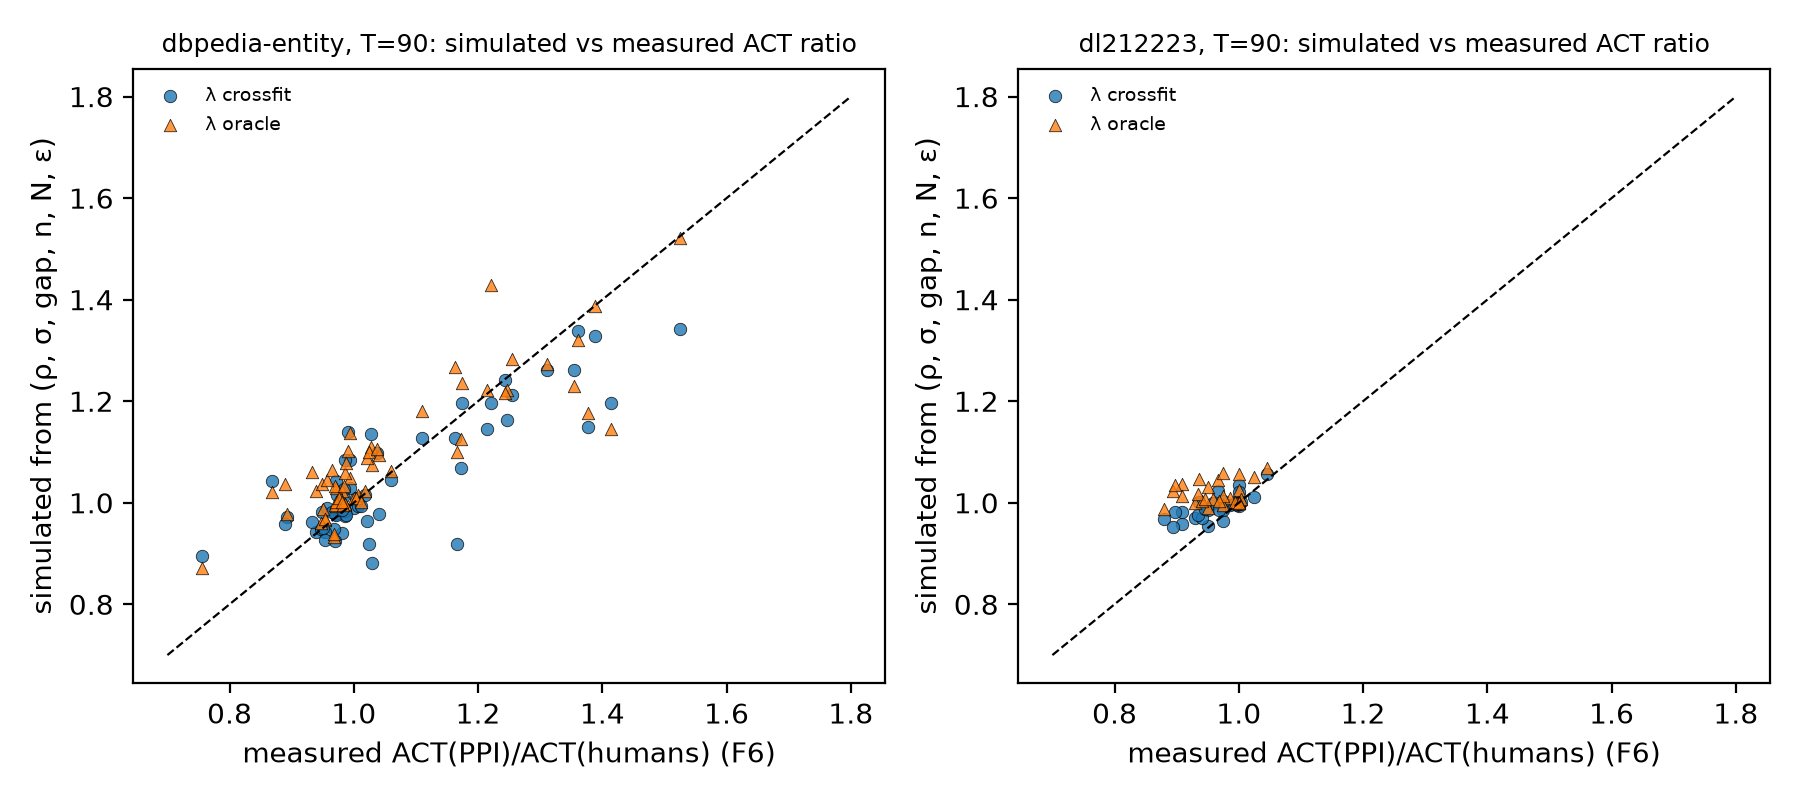
\includegraphics[width=0.9\linewidth]{figures/F9_calculator.png}
\caption{Simulated against measured $\ACT$ ratio, $T=90$, every cell of Figure~\ref{fig:F6}; circles use the cross-fitted $\lambda$ of the implementation, triangles the population-optimal $\lambda$. Left DBpedia-Entity, right TREC DL 2021--23.}\label{fig:F9}
\end{figure}

\section{Reproducibility notes}\label{app:repro}
All numbers are regenerated from row-level result files by the scripts in the repository (the revised cost table by \texttt{86\_table2\_v2.py} from the \texttt{\_v2} result files; the cost model of Appendix~\ref{app:costmodel} by \texttt{95\_cost\_model.py}; the menu-allocation and exact-certificate appendices from \texttt{83\_menu\_allocation.py} and \texttt{63\_planner\_v2.py} with the options recorded in the design log; the pilot-size table by \texttt{88\_pilot\_sweep.py} from the \texttt{--n\_train} and \texttt{--fixed\_cand} runs of \texttt{83}). Each method uses an independent random stream derived from the repeat index and the method name. Batched causal-LM inference with left padding must pass explicit position ids; without them the relevance judgments on one collection (TREC-COVID) collapsed to a constant, which we detected from a 49/50-query anomaly, fixed, and re-ran for every collection (label changes $\le0.5\%$ elsewhere; reranker scores unaffected, checked against batch-size-1 scoring). The BCa lower bound on $\rho$ used by the adoption rule covered its target at $0.88$--$0.92$ for pilots of 30 and 50 queries on DBpedia-Entity ($0.86$ at 20), against $0.75$--$0.84$ for the Fisher-$z$ bound on skewed pairs. The lock documents for Section~\ref{sec:prereg} were written before the target data were accessed (the only pre-lock access was the count of judged queries and pairs). The public repository's history, however, begins with a single release commit that already contains the lock documents together with the results, so the ordering is documented by the dated lock files and the development log rather than by the public commit sequence; a reader who needs independent evidence of the timing should treat the pre-registration as self-reported.
\end{document}
